\documentclass[10pt]{amsart}
\usepackage[margin=1.05in]{geometry}
\addtolength{\oddsidemargin}{-.1in} 
\usepackage{amsmath,amsthm,amssymb}
\usepackage{bm}
\usepackage{enumitem}
\usepackage{array}
\usepackage{lipsum}
\usepackage[]{units}
\usepackage{relsize}
\usepackage{verbatim}
\usepackage{bbm}
\usepackage{stackengine}
\usepackage{amsthm}
%\usepackage{hyperref}



\newtheoremstyle{cited}%
  {3pt}% (space above)
  {3pt}% (space below)
  {\itshape}% (body font)
  {}% (indent amount)
  {\bfseries}% {theorem head font}
  {.}% {punctuation after theorem head}
  {.5em}% {space after theorem head}
  {\thmname{#1} \thmnumber{#2} \thmnote{\normalfont#3}}% {theorem head spec}


\usepackage{tikz}
\usetikzlibrary  {positioning}
\usepackage{graphicx}
\usepackage{xfrac}
%\usetikzlibrary{cd}
\usepackage{tikz-cd}
\usepackage{tkz-berge}
\usetikzlibrary{shapes,snakes}
\usetikzlibrary{decorations.markings}


\setenumerate{listparindent=\parindent}

\newcommand{\M}{\mathcal{M}}
\newcommand{\B}{\mathcal{B}}
\renewcommand{\S}{\mathcal{S}}
\newcommand{\Q}{\mathbb{Q}}
\newcommand{\Z}{\mathbb{Z}}
\newcommand{\R}{\mathbb{R}}
\newcommand{\C}{\mathbb{C}}
\renewcommand{\H}{\mathbb{H}}
\renewcommand{\O}{\mathbb{O}}
\renewcommand{\L}{\mathbf{L}}
\newcommand{\HH}{\mathbf{H}}
\newcommand{\G}{\mathbf{G}}
\newcommand{\K}{\mathbf{K}}
\newcommand{\omd}{\omega_{\scriptscriptstyle D}}



\newcommand{\p}{\mathfrak{p}}
\newcommand{\q}{\mathfrak{q}}
\renewcommand{\a}{\mathfrak{a}}
\renewcommand{\b}{\mathfrak{b}}
\renewcommand{\c}{\mathfrak{c}}
\renewcommand{\o}{\mathfrak{o}}
\newcommand{\m}{\mathfrak{m}}
\renewcommand{\d}{\mathfrak{d}}
\newcommand{\gen}[1]{\langle #1 \rangle}
%\let\oldref\ref
%\renewcommand{\ref}[1]{\oldref{#1}}



\DeclareMathOperator*{\dom}{dom}
\DeclareMathOperator*{\Aut}{Aut}
\DeclareMathOperator*{\Ann}{Ann}
\DeclareMathOperator*{\Tor}{Tor}
\DeclareMathOperator*{\Gal}{Gal}
\DeclareMathOperator*{\Hom}{Hom}
\DeclareMathOperator*{\End}{End}
\DeclareMathOperator*{\im}{Im}
\DeclareMathOperator*{\re}{Re}
\let\ker\relax
\DeclareMathOperator*{\ker}{Ker}
\DeclareMathOperator*{\Emb}{Emb}
\renewcommand{\bar}{\overline}

\newcommand{\thefield}{\Q(\sqrt{-D})}
\newcommand{\thering}{\mathcal{O}_{\Q(\sqrt{-D})}}
\newcommand{\Ord}{\mathcal{O}}
\newcommand{\norm}[1]{\left[#1\right]}


%\theoremstyle{cited}
\newtheorem{thm}{Theorem}
\newtheorem{lem}[thm]{Lemma}
\newtheorem{defn}[thm]{Definition}
\newtheorem{prop}[thm]{Proposition}
\newtheorem{cor}[thm]{Corollary}
\newtheorem{ex}[thm]{Example}
\newtheorem{conj}[thm]{Conjecture}






%Inline equation
\newcommand*{\inlineequation}[2][]{%
  \begingroup
    % Put \refstepcounter at the beginning, because
    % package `hyperref' sets the anchor here.
    \refstepcounter{equation}%
    \ifx\\#1\\%
    \else
      \label{#1}%
    \fi
    % prevent line breaks inside equation
    \relpenalty=10000 %
    \binoppenalty=10000 %
    \ensuremath{%
      % \displaystyle % larger fractions, ...
      #2%
    }%
    ~\@eqnnum
  \endgroup
}
\makeatother


\makeatletter
\let\@@pmod\pmod
\DeclareRobustCommand{\pmod}{\@pmods}
\def\@pmods#1{\mkern4mu({\operator@font mod}\mkern 6mu#1)}
\makeatother


\title{Lattice Embeddings in the Composition Algebras}
\author{Michael Knopf, UC Berkeley}
\date{December 10, 2015}

\begin{document}
\maketitle
\noindent
I would like to thank Professor George Bergman for advising this paper, especially for his patient reading and many helpful suggestions.

\begin{abstract}
Define a \emph{rational composition algebra} to be a Euclidean Hurwitz algebra, except where the underlying field is $\Q$.  I prove a simple characterization of all such algebras.  One example is the subring $\Q(i,j) \subset \H$ of quaternions with rational coordinates, which can be identified with $\Q^4$.  The Hurwitz integral quaternions $\HH$ are a maximal order of algebraic integers in $\Q(i,j)$.  If $\M$ is a subset of $\R^n$ with the squared distance between any two points integral, call $\M$ an \emph{integer norm set}.  If $\M \subset \Q(i,j)$ is an integer norm set, I prove there is an inner automorphism of $\Q(i,j)$ for which the image of $\M$ lies in $\HH$.  In particular, every order of algebraic integers in $\Q(i,j)$ is isomorphic to a subring of $\HH$.  If $\M \subset \R^2$ is an integer norm set, not necessarily in $\Q(i,j)$, there is a positive squarefree integer $D$ such that any triangle formed in $\M$ has area of the form $q\sqrt{D}$ for some $q \in \Q$.  I prove that if $D \not \equiv 3 \pmod{4}$, $\M$ embeds congruently in $\Z^4$; and if $D \not \equiv 7 \pmod{8}$, $\M$ embeds congruently in $\HH$.  If $D \equiv 7 \pmod{8}$, I conjecture that $\M$ embeds congruently in the Kleinian octaves, an order within the octonion algebra.  This conjecture would imply that all integer norm sets in $\R^2$ embed in the \emph{Double Hurwitzian Ring} $\HH \oplus \HH$.
\end{abstract}

\section{Introduction}

A well-known problem of Paul Erd\"os asks for $n$ points in the plane, no three on a line and no four on a circle, for which all pairwise distances are integral.  A point set of this kind is said to be in ``general position".  In 2008, it was announced that a set of seven such points had been found, having a diameter of $22270$ \cite{Kr08}.  When coordinates for this heptagon were presented, they had the curious property that each point was of the form $(a,b\sqrt{2002})$ for integers $a$ and $b$.

This phenomenon is no coincidence.  In fact, the number $2002$ turns out to be a defining feature of this point set: any $3$ of its points form a triangle with area of the form $\frac{z}{4}\sqrt{2002}$, where $z$ is an integer.  In general, if $\M \subseteq \R^2$ is a set of points in the plane such that $|x-y|^2 \in \Z$ for all $x,y \in \M$, then there exists a squarefree integer $D$ such that any three points in $\M$ form a triangle of area $\frac{z}{4}\sqrt{D}$ for some integer $z$.  If $\M$ is not collinear, the number $D$ is called the $\emph{characteristic}$ of $\M$ \cite{Kr08}.  We call such a set a \emph{planar integer norm set}.

Naturally, the case of $D=1$ has been of interest, and it has been shown that $\M$ embeds in $\Z^2$ if this holds (when we speak of embeddings, we will always mean congruent embeddings via an isometry) \cite{Yi17,Fr01,Lu12,Ma13}.  The general case was explored and it was established that, when the square of every ideal of $\thering$(the maximal order of algebraic integers within $\Q(\sqrt{-D})$) is principal, $\M$ embeds in $\thering$ if it embeds in $\thefield$; conversely, if the square of some ideal is nonprincipal, then there exists such a pointset - a triangle, even - which embeds in $\thefield$ but not in $\thering$.  It is natural to consider such lattices as targets for these embeddings, for if $\M$ has characteristic $D$ then it cannot embed in $\Q(\sqrt{-E})$ for any squarefree $E \neq D$ \cite{Kn15}, but a simple condition can be given to characterize whether $\M$ embeds in $\Q(\sqrt{-D})$.

This paper investigates the remaining cases of those $\M$ for which no embedding in $\thering$ exists, as well as integer norm sets which are not planar.  Clearly, any subset of $\thering$ is an planar integer norm set, nevertheless not all planar integer norm sets can be realized as subsets of one of these orders.  Is there a natural lattice that does have this property?  I conjecture that the answer is yes, and that the lattice we seek is the double Hurwitzian ring, a sublattice of the integral octonions.

In an effort to keep this paper as self-contained as possible, I have presented all background material necessary to understand the final results.  Sections 4, 7, and 8 contain primarily new material; anything in these sections that has been proven before will be clearly attributed.  Section 3 contains an original presentation of some elementary concepts of this theory, which are certainly well-known.  Proposition \ref{prop:finite} is a key result that I have not found in the literature, but I am certain would also be considered elementary.

%%%%%%%%%%%%%%%%%%%%%%%%%%%%%%%%%%%%%%%%%%%%%%%%%

\section{The Composition Algebras}

\noindent
\textbf{Note:} The appendix contains a collection of laws satisfied in a composition algebra.  They are labeled by a letter followed by a number.  For instance, the ``braid law", which states that $\norm{\alpha\beta, \gamma} = \norm{\beta, \bar{\alpha}\gamma}$ is labeled C1.  When one of these relations is used, we will indicate this by placing its label over an equality sign.  For example, $\norm{\alpha(\gamma\delta),\beta\nu} \overset{\text{C1}}{=} \norm{\gamma\delta, \bar{\alpha}\beta\nu}$.

\begin{defn}
\normalfont
An \emph{algebra over a field} is a vector space $V$, over a field $K$, equipped with a bilinear, not necessarily associative, multiplication $V \times V \rightarrow V$.
\end{defn}

In general, an inner product space is usually thought of to have $\R$ or $\C$ as its underlying field.  We will do away with this convention, and allow an inner product space to use $\Q$ as its field of scalars.  For the purposes of this paper, we adopt the following definition, though outside this discussion this object might instead be called a ``Euclidean Hurwitz algebra":

\begin{defn} \label{def:comp}
\normalfont
Let $V$ be a finite-dimensional inner product space over a field $F$, where $F = \Q$ or $F = \R$, with inner product $\norm{\ \cdot \ ,\ \cdot \ } : V \times V \rightarrow F$.  Define a \emph{norm} function $\norm{\ \cdot \ } : V \rightarrow F$ by $\norm{\alpha} = \norm{\alpha,\alpha}$.  Suppose we define a multiplication making $V$ into a unital algebra $A$ over $F$.  Then $A$ is called a \emph{composition algebra} if the identity
$$
\norm{\alpha \beta} = \norm{\alpha}\norm{\beta}
$$
holds, which is known as the \emph{composition law}.  We call a composition algebra $A$ a \emph{rational composition algebra} if $F = \Q$ and a \emph{real composition algebra} if $F = \R$.
\end{defn}

We will follow the convention of using Greek letters for elements of a composition algebra and Roman letters for real numbers.  We call $\norm{\alpha,1}$ the \emph{real part} of $\alpha$, and denote it by $\re(\alpha)$.  We also define a conjugation operator by $\bar{\alpha} = 2[\alpha,1] - \alpha$.  It is verified, in the appendix, that the identities $\bar{\alpha + \beta} = \bar{\alpha} + \bar{\beta}$, $\bar{\alpha \cdot \beta} = \bar{\beta} \cdot \bar{\alpha}$, $\bar{\bar{\alpha}} = \alpha$, and $\alpha \bar{\alpha} = \norm{\alpha}$ are satisfied.  If $A$ and $B$ are composition algebras over $F$, we define an \emph{embedding of $A$ into $B$} to be an inner product space homomorphism $\varphi$ such that $\varphi(1) = 1$ and $\varphi(\alpha\beta) = \varphi(\alpha)\varphi(\beta)$ for all $\alpha, \beta \in A$.  By saying $\varphi$ is an inner product space homomorphism, we mean that $\varphi$ is a linear map satisfying $\norm{\varphi(\alpha),\varphi(\beta)} = \norm{\alpha,\beta}$ for all $\alpha, \beta \in A$.  Therefore, an embedding of composition algebras must be injective, since $\varphi(\alpha) = 0$ if and only if $\norm{\varphi(\alpha)} = \norm{\alpha} = 0$, which is equivalent to having $\alpha = 0$.  If an embedding of composition algebras is surjective as well, call it an \emph{isomorphism of composition algebras}.  This leads us to the following simplification:

\begin{prop} \label{prop:R^n}
\normalfont
Up to isomorphism, any real composition algebra is the inner product space $\R^n$, with the standard Euclidean inner product, equipped with some bilinear multiplication.
\end{prop}

\begin{proof}
If $A$ is a composition algebra space over $\R$ of finite dimension $n$, we can extend $\{1\} \subseteq A$ to a basis of $A$, then apply the Gram-Schmidt process to obtain an orthonormal basis.  It follows that $A$ is isomorphic, as an inner product space, to $\R^n$ with the standard Euclidean inner product.  This isomorphism can be chosen to send $1_A$ to $e_1 \in \R^n$.  The linearity of the isomorphism then induces a bilinear multiplication on $\R^n$ satisfying the composition law, making it into an algebra isomorphic to $A$.
\end{proof}


Obviously, $\R$ itself is a real composition algebra, though the quintessential example is $\C$.  Still well-known is the ring of quaternions $\H$, which extends $\C$ by adjoining an orthogonal unit vector $j$ and imposing the relations $i^2 = j^2 = k^2 = ijk = -1$, where $k = ij$.  A consequence of this definition is that $k$ is orthogonal to $1,i$, and $j$, but together these four vectors span all of $\H$.

To obtain a final example, we repeat this process, this time adjoining an element orthogonal to $\H$ and defining a multiplication in the following way: denote the basis elements of $\H$ by $i_\infty = 1$, $i_0 = i$, $i_1 = j$, $i_3 = ij$, and call the new orthogonal element $i_2$.  Next, define $i_4 = i_1i_2$, $i_5 = i_2i_3$, and $i_6 = i_3i_4$.  These $8$ elements are pairwise-orthogonal, and their multiplication is given by the relations
\begin{align*}
&i_n^2 = -1 \\
&i_\infty i_n = i_n =  i_n i_\infty \\
&i_{n+1}i_{n+2} = i_{n+4} = - i_{n+2}i_{n+1} \\
&i_{n+2}i_{n+4} = i_{n+1} = - i_{n+4}i_{n+2} \\
&i_{n+4}i_{n+1} = i_{n+2} = - i_{n+1}i_{n+4}
\end{align*}
for $0 \leq n \leq 6$, where the indices are taken mod $7$.  $\O$ fails to be associative.  However, it is \emph{alternative}, meaning that $\alpha(\alpha\beta) = \alpha^2 \beta$ for all $\alpha,\beta \in \O$.  A theorem of Artin states that the subalgebra generated by two elements in an alternative algebra is associative.

Notice that any pair of the elements $i_a, i_b$, for $a,b \neq \infty$, generate a quaternion subalgebra, since any $r,s \in \Z_7$ differ by either $1$,$2$, or $3$ (in absolute value), thus the algebra they generate is determined by the above relations after fixing an appropriate $n$ for the bottom three relations.  For example, $i_3$ and $i_5$ generate the algebra $\R[i_2,i_3,i_5]$, whose multiplication is found by fixing $n = 1$.  Furthermore, all quaternion subalgebras having $\{i_\infty, i_a, i_b, i_c\}$ as a basis over $\R$, for some distinct $a,b,$ and $c$, arise by fixing some $n$ in these relations.  For if $c$ were not the index such that $i_a i_b = \pm i_c$, then the space spanned by $\{i_\infty, i_a, i_b, i_c\}$ would not be closed under multiplication.

%This means that all quaternion subalgebras using some choice of four of these standard basis vectors are found by choosing 2 of the 7 imaginary components.  However, each of these subalgebras can be created in $\binom{3}{2}$ ways by this process, since any two of $n, n+1,$ and $n+3$ yield the same result, for each $n$.  Thus, there are exactly $\binom{7}{2} / \binom{3}{2} = 7$ quaternion subalgebras with a basis of this form.

The phenomenon just observed can be visualized by labeling the vertices of the Fano plane, as shown below, and identifying each line with the quaternion subalgebra generated by the units corresponding to the nodes it passes through.  The direction of each line symbolizes the ``positive direction of multiplication."  For instance, $i_5i_2 = i_3$, but $i_2i_5 = -i_3$ is visualized by the direction of the line connecting $5$, $2$, and $3$.

\tikzset{->-/.style={decoration={
  markings,
  mark=at position #1 with {\arrow{>}}},postaction={decorate}}}

\tikzset{-<-/.style={decoration={
  markings,
  mark=at position #1 with {\arrow{<}}},postaction={decorate}}}

\begin{center}
\begin{tikzpicture}[scale = 3]

\draw[->-=.2] (0,0) circle (0.5);
   %\draw (90:1) -- (-30:1)--(210:1) -- cycle;
   
\draw[-<-=.2] (90:1) -- (-30:1);
\draw[-<-=.2] (-30:1)--(210:1);
\draw[-<-=.2] (210:1) -- (90:1);

   \draw (90:1)--(0,0);
   \draw (210:1)--(0,0);
   \draw (-30:1)--(0,0);

   \draw[-<-=.5] (30:0.5)--(0,0);
   \draw[-<-=.5] (150:0.5)--(0,0);
   \draw[-<-=.5] (270:0.5)--(0,0);

	

   \fill[white] (-0.866,-0.5) circle (3pt);
   \node[draw, circle] at (-0.866,-0.5) {$3$};
   
   \fill[white] (0.866,-0.5) circle (3pt);
   \node[draw, circle] at (0.866,-0.5) {$6$};
   
   \fill[white] (0,-0.5) circle (3pt);
   \node[draw, circle] at (0,-0.5) {$4$};
   
   \fill[white] (0,1) circle (3pt);
   \node[draw, circle] at (0,1) {$5$};
   
   \fill[white] (0,0) circle (3pt);
   \node[draw, circle] at (0,0) {$0$};
   
   \fill[white] (0.433,0.25) circle (3pt);
   \node[draw, circle] at (0.433,0.25) {$1$};
   
   \fill[white] (-0.433,0.25) circle (3pt);
   \node[draw, circle] at (-0.433,0.25) {$2$};
\end{tikzpicture}
\end{center}



The above process of extending an algebra by adjoining an orthogonal vector and imposing multiplicative relations that result in a composition algebra is called the Cayley-Dickson construction.  A subtly different situation is one in which $H$ is a proper subalgebra of a larger composition algebra.  In this case, there is already a natural extension of $H$ found by choosing an element $i$ orthogonal to $H$ and forming the subalgebra $H+iH$.  This algebra is unique up to isomorphism, since its multiplication is completely determined by the composition doubling law (D3).  We call $H + iH$ the ``Dickson double" of $H$.  In light of the following famous theorem, the Cayley-Dickson construction must terminate after three doublings of the base field $\R$.  Important details of the proof, borrowed from \cite{Co03}, are relegated to the appendix, but the key ideas are all contained here.

\begin{thm}[Hurwitz]
\normalfont
The only real composition algebras are $\R$, $\C$, $\H$, and $\O$.
\end{thm}

\begin{proof}[Sketch of proof]
Let $Y$ be a real composition algebra, and suppose it contains a proper sub-algebra $X$.  Then $Y$ contains an element orthogonal to $X$ and thus also contains its Dickson double.  In fact, since $Y$ is finite-dimensional it must itself be a Dickson double, for otherwise it would lie strictly between a proper subalgebra and its Dickson double.

Suppose then that $Y = X + i_Y X$, where $X \subsetneq Y$ and $i_Y \in Y$ is a unit vector orthogonal to $X$.  It follows from the composition law alone (see (D3) in the appendix) that
$$
(a+i_Yb)(c+i_Yd) \overset{\text{D3}}{=} (ac-d\bar{b}) + i_Y(cb+\bar{a}d)
$$
for all $a,b,c,d \in X$.  Therefore, we must have, for all $a,b,c,d \in X$,
$$
\norm{a+i_Yb}\norm{c+i_Yd} = \norm{(ac-d\bar{b}) + i_Y(cb+\bar{a}d)}.
$$
Expanding this expression and canceling, we see that $[ac,d\bar{b}] = [cb,\bar{a}d]$, or equivalently $[(ac)b,d] \overset{\text{C1}}{=} [a(cb),d]$, holds for all $a,b,c,d \in X$.  This implies the law of associativity for $X$.  Thus, $X$ is an associative composition algebra.

Suppose a real composition algebra is not $\R, \C,$ or $\H$.  The algebra is unital, and thus properly contains $\R$.  By Dickson doubling, it must then contain $\C$, $\H$, and $\O$ as well.  If the containment of $\O$ were proper, it would also contain its Dickson double, contradicting that it is a composition algebra because $\O$ is nonassociative.  Therefore, the algebra must be $\O$.
\end{proof}

\noindent For a more detailed overview of these topics, refer to \cite{Co03} or the appendix.

\section{Automorphisms of $\O$}

The Cayley-Dickson construction gives us a method of understanding the automorphism groups of real composition algebras.  Let $\{\alpha, \beta, \gamma\} \subset \O$ be a set of unit length vectors such that $\alpha \perp \R$, $\beta \perp \R(\alpha)$, and $\gamma \perp \R(\alpha,\beta)$.  In the Cayley-Dickson construction, we could have chosen $\alpha$ to be the vector which extends $\R$ to $\C$, then $\beta$ to be the vector which extends $\C$ to $\H$, and finally $\gamma$ to be the vector which extends $\H$ to $\O$.  Therefore, the map $i_0 \mapsto \alpha, i_1 \mapsto \beta, i_2 \mapsto \gamma$ induces an automorphism of $\O$. 

Conversely, if $\varphi$ is an automorphism of $\O$, and we let $\alpha = \varphi(i_0), \beta = \varphi(i_1)$, and $\gamma = \varphi(i_2)$, then it is necessarily the case that none of $\alpha$, $\beta$, and $\gamma$ are in the algebra generated by either of the other two over $\R$.  For the algebra generated by any two over $\R$ must be, by the Cayley-Dickson construction, isomorphic to $\H$.  If this subalgebra were to contain the third element as well, then it would have to be all of $\O$, and clearly $\O$ cannot be embedded into $\H$, since it has greater dimension.  Therefore, $\{\alpha, \beta, \gamma\} \subset \O$ must be a set of unit length vectors such that $\alpha \perp \R$, $\beta \perp \R(\alpha)$, and $\gamma \perp \R(\alpha,\beta)$.  Thus, the set of automorphisms of $\O$ is in correspondence with sets of the form $\{\alpha, \beta, \gamma\} \subset \O$ where $\norm{\alpha} = \norm{\beta} = \norm{\gamma} = 1$ and $\alpha \perp \R$, $\beta \perp \R(\alpha)$, and $\gamma \perp \R(\alpha,\beta)$

Similarly, by choosing any two elements $\alpha, \beta \in \O$ of unit length satisfying with $\alpha \perp \R$ and $\beta \perp \R(\alpha)$, we can create an embedding $\H \hookrightarrow \O$ by $i \mapsto \alpha, j \mapsto \beta$.  Conversely, any such embedding must be of this form.  Therefore, the set of embeddings of $\H$ into $\O$ are in correspondence with sets of the form $\{\alpha, \beta\} \subseteq \O$ where $\norm{\alpha} = \norm{\beta} = 1$, $\alpha \perp \R$, and $\beta \perp \R(\alpha)$.   Continuing this reasoning, we see that the set of embeddings of $\C$ into $\O$ is in correspondence with the set of elements of $\O$ of unit length that are orthogonal to $\R$.  This establishes the following theorem:

\begin{thm} \label{thm:autom}
\normalfont
Let $\S_1, \S_2, \S_3$ be the collections of every subset of $\O$ that is a minimal orthonormal generating set for a subalgebra isomorphic to $\C$, $\H$, or $\O$, respectively.  That is, for each $n \in \{1,2,3\}$, define
$$
\mathcal{S}_n = \{
\{\alpha_1,\dots,\alpha_n\} \subset \O : r,s,t \in \{1,\dots,n\}, r \not \in \{s,t\}, \alpha_r \not \in \R(\alpha_s,\alpha_t)\}.
$$
The maps $\Emb(\C, \O) \rightarrow \mathcal{S}_1$ defined by $\varphi \mapsto \{\varphi(i)\}$, $\Emb(\H,\O) \rightarrow \mathcal{S}_2$ defined by $\varphi \mapsto \{\varphi(i_0), \varphi(i_1)\}$, and $\Aut(\O) \rightarrow \mathcal{S}_3$ defined by $\varphi \mapsto \{\varphi(i_0),\varphi(i_1),\varphi(i_2)\}$ are bijections.
\end{thm}

\begin{cor}[Diassociativity]
\normalfont
A subalgebra of $\O$ generated by two elements is associative.
\end{cor}
\begin{proof}
The subalgebra generated by any two elements of $\O$ is isomorphic to $\R$, $\C$, or $\H$.
\end{proof}

Let $A$ be an algebraic structure with a binary operation and an inverse operator, written additively. Let $I$ be an index set.  A \emph{generalized permutation} is an operation on $\prod_{t \in I} A$ of the form
$$
\prod_{t \in I} x_i \mapsto \prod_{t \in I}\lambda_t (x_{\sigma^{-1}(t)})
$$
where the function $\lambda: I \rightarrow \{\text{id}, x \mapsto -x\}$ assigns, to each element $t \in I$, a function $\lambda_t$ which is either the identity map on $A$ or the inverse map on $A$, and $\sigma$ is a permutation of $I$.  Less formally, a generalized permutation is an operation on $\prod_{t \in I} A$ that ``permutes components change signs."  For a given generalized permutation, we will call $\lambda$ the \emph{associated sign function} and $\sigma$ the \emph{associated permutation}.  Consider the following example: $(a,b,c) \mapsto (-c,a,b)$ is a generalized permutation on $A^3$ with associated sign function defined by $1 \mapsto (x \mapsto -x)$, and $2,3 \mapsto \text{id}$, and associated permutation defined by $1 \rightarrow 2 \rightarrow 3 \rightarrow 1$.

If $f$ and $g$ are two generalized permutations on $\prod_{t \in I} A$, with associated sign functions $\lambda$ and $\mu$, and associated permutation $\sigma$ and $\tau$, then $f \circ g$ is a generalized permutation on $\prod_{t \in I} A$ with associated sign function $\nu$, where $\nu_t = \lambda_t \circ \mu_t$ for each $t \in I$, and associated permutation $\sigma\tau = \sigma \circ \tau$.  Generalized permutations are clearly invertible.  Since function composition is associative, the generalized permutations on $\prod_{t \in I}$ form a group $G \cong \Z_2 \times \text{Perm}(I)$, and the map taking a generalized permutation on $\prod_{t \in I} A$ to its associated permutation is a homomorphism from $G$ to the group of permutations on $I$.

Let $\Omega = \{\infty,0,1,2,3,4,5,6\}$, so that $\O \cong \prod_{t \in \Omega}\R$.  Every element $\gamma \in \O$ induces left and right multiplication operators $L_\gamma$ and $R_\gamma$ on $\O$, defined in the obvious way.  If $\gamma = i_r$ for some $r \in \Omega$, then these operators are generalized permutations on $\O$ when it is viewed as $\R^8$.  Fix some $r \in \Omega$ and assume $M_{i_r}$ is one of $L_{i_r}$ or $R_{i_r}$, since the arguments we will use for one apply to both.  Note that, for $t \in \Omega$, $\sigma$ is the permutation associated with $M_{i_t}$ if and only if
$$
M_{i_t}\left( \sum_{s \in \Omega} a_s i_s \right) = \sum_{s \in \Omega} a_{\sigma^{-1}(s)} i_s = \sum_{s \in \Omega} a_s i_{\sigma(s)}.
$$


If $S$ is a subset of $\Omega$ containing $r$ then, by closure under multiplication, $M_{i_r}$ restricts to a generalized permutation on $\R(\{i_t : t \in S\})$ (when it is viewed as a direct product of copies of $\R$).  Less obvious is the following fact.

\begin{prop} \label{prop:genperm}
\normalfont
If $S$ is a 4-element subset of $\Omega$ such that $\R(\{i_t : t \in S\}) \cong \H$ and $r \in S^c = \Omega \setminus S$, then $\sigma(S) = S^c$ and $\sigma(S^c) = S$, where $\sigma$ is the associated permutation of $M_{i_r}$.
\end{prop}

\begin{proof}
To see this, first check the claim for $S = \{ \infty, 0, 1, 3\}$ and $r = 2$:

\begin{align*}
L_{i_2}(a i_\infty +  b i_0 + c i_1 + d i_3) &= ai_2 - bi_6 - ci_4 + d i_5 \\
R_{i_2}(a i_\infty +  b i_0 + c i_1 + d i_3) &= ai_2 + bi_6 + ci_4 - d i_5
\end{align*}

If $S'$ is another 4-element subset of $\Omega$ such that $\R(\{i_t : t \in S'\}) \cong \H$ and $r' \not \in S$, then by Theorem~\ref{thm:autom} there is a permutation $\tau$ of $\Omega$ taking $S'$ to $S$ (note that this implies $\tau(S'^c) = S^c$ as well) and $r'$ to $r$ that induces an automorphism $\varphi_{\tau}$ of $\O$, defined by
$$
\varphi_{\tau}\left( \sum\limits_{s \in \Omega} a_s i_s \right) = \sum\limits_{s \in \Omega} a_s i_{\tau(s)}.
$$
More formally, we know that $\R(\{i_t : t \in S\}) = \R(i_{t_1}, i_{t_2}) \cong \H$ and $\R(\{i_t : t \in S'\}) = \R(i_{t_1}', i_{t_2}') \cong \H$ for some $t_1,t_2,t_1',t_2' \in \Omega$ with $t_1 \neq t_2$ and $t_1' \neq t_2'$.  Therefore, the map $i_{t_1} \mapsto i_{t_1}', i_{t_2} \mapsto i_{t_2}'$ induces an embedding of $\R(\{i_t : t \in S\})$ into $\R(\{i_t : t \in S'\})$.  It can then be extended to an automorphism of $\O$ simply by choosing an image for $i_r$ that is orthogonal to $\R(\{i_t : t \in S'\})$, since $i_r \perp \R(\{i_t : t \in S\})$.  We know that $i_r' \perp \R(\{i_t : t \in S'\})$, thus $i_r'$ is a valid choice.

$\varphi_{\tau}$ is also a generalized permutation on $\O$, with associated permutation $\tau$.  Also, $\varphi_{\tau}^{-1} = \varphi_{\tau^{-1}}$ has associated permutation $\tau^{-1}$.
We now have the following commutative squares

$$
\begin{tikzpicture}[baseline= (a).base]
\node[scale=1.3] (a) at (0,0){

\begin{tikzcd}
\O \arrow{dd}[swap]{M_{i_{\tau(r)}}} \arrow{rr}{\varphi_\tau} & & \O \arrow{dd}{M_{i_{r}}} \\
& & & \\
\O \arrow{rr}[swap]{\varphi_\tau} & & \O
\end{tikzcd}

};


\begin{scope}[shift={(7,0)}]
\node[scale=1.3] (a) at (0,0){

\begin{tikzcd}
S' \arrow{dd}[swap]{\tau^{-1}  \sigma  \tau} \arrow{rr}{\tau} & & S \arrow{dd}{\sigma} \\
& & & \\
S'^c \arrow{rr}[swap]{\tau} & & S^c
\end{tikzcd}
};
\end{scope}
\end{tikzpicture}
$$
The commutativity of the left diagram follows from
$$
\varphi_{\tau}\circ L_{i_r} ( \alpha) = \varphi_{\tau}(i_r \alpha) = \varphi_{\tau}(i_r)\varphi_{\tau}(\alpha) = i_{\tau(r)} \varphi_\tau(\alpha) = L_{i_{\tau(r)}}\circ \varphi_\tau (\alpha)
$$
and
$$
\varphi_{\tau}\circ R_{i_r} ( \alpha) = \varphi_{\tau}(\alpha i_r) = \varphi_{\tau}(\alpha)\varphi_{\tau}(i_r) = \varphi_\tau(\alpha) i_{\tau(r)} = R_{i_{\tau(r)}}\circ \varphi_\tau (\alpha).
$$
The associated permutation of $M_{i_{\tau(r)}} = \varphi_{\tau}^{-1} \circ M_{i_r} \circ \varphi_{\tau}$ is $\tau^{-1}\sigma\tau$, which has the desired properties $\tau^{-1}\sigma\tau(S') = S'^c$ and $\tau^{-1}\sigma\tau(S'^c) = S'$.  Therefore, the proposition holds for an arbitrary halving set $S$ and $r \in S^c$.
\end{proof}


\section{Rational Composition Algebras}

An observation regarding rational composition algebras can be made that is similar to Proposition~\ref{prop:R^n}.

\begin{lem} \label{lem:rat}
\normalfont
Let $Q$ be a rational composition algebra.  Then $Q$ has an orthogonal basis, and there is a unique extension of $Q$ to a real composition algebra.
\end{lem}
\begin{proof}
If $V$ is an inner product space over $\Q$ of finite dimension $n$, then a modified version of the Gram-Schmidt process produces an orthogonal (not necessarily orthonormal) basis as follows.  Choose a basis $\{v_1, \dots , v_n\}$ for $V$ over $\Q$.  Suppose that we have found a pairwise orthogonal list $\{u_1, \dots , u_k\}$, with $1 \leq k < n$, that spans the same subspace as $\{v_1, \dots , v_k\}$.  Define
$$
u_{k+1} = v_{k+1} - \frac{\norm{v_{k+1}, u_1}}{\norm{u_1}} u_1 - \cdots - \frac{\norm{v_{k+1}, u_k}}{\norm{u_k}} u_k.
$$
Taking the inner product of $u_{k+1}$ with any of $u_1, \dots , u_k$ shows that adding $u_{k+1}$ to this list produces a new list that is still pairwise orthogonal.  Repeating this process will eventually yield an orthogonal basis.  Thus, $Q$ has an orthogonal basis.

Taking an orthogonal basis $\{\beta_1, \dots , \beta_n\}$ for $Q$, we may embed $Q$ as a subset of $\R^n$ by the linear map induced by $\beta_j \rightarrow 
\sqrt{\norm{\beta_j}}e_j$, where $e_j$ is the $j$th standard basis vector in $\R^n$.  For now, we will simply identify $Q$ with this subset, noting that the inner product on $Q$ is the restriction of the standard Euclidean inner product to this subset.

The Euclidean distance on $\R^n$, which is the squareroot of $Q$'s norm function, makes $Q$ into a metric space.  This metric induces the product metric on $Q \times Q$.  Fix a value $\beta \in Q$, and let $\alpha_k$ be a Cauchy sequence in $Q$.  We aim to show that $\alpha_k \beta$ is Cauchy as well, showing that the right multiplication map is continuous.  This is obvious if $\beta = 0$, so assume otherwise.  Given $\epsilon > 0$, there is some $N$ such that $|\alpha_j - \alpha_k| < \frac{\epsilon}{|\beta|}$ whenever $j,k > N$.  From the composition law in $Q$, we have
$$
|\alpha_j \beta - \alpha_k \beta| = |\alpha_j - \alpha_k||\beta| < \epsilon
$$
whenever $j,k > N$, and so the result follows.  A symmetric argument shows that the left multiplication map is continuous, as well.  Therefore, the multiplication map $Q \times Q \rightarrow Q$ is continuous, because it is continuous in both of its components.

Since $Q$ is a rational vector space of dimension $n$ embedded in $\R^n$, it is dense in $\R^n$.  Thus we may, for any $\alpha,\beta \in \R^n \setminus Q$, take a sequence $(\alpha_k, \beta_k)$ in $Q \times Q$ converging to $(\alpha, \beta)$.  By the continuity of multiplication, $\alpha_k \beta_k$ is Cauchy, and so converges to some point in $\R^n$.  Define the product $\alpha\beta$ to be this point.  The composition law holds for $\alpha$ and $\beta$ because the distance function is continuous, thus
$$
|\alpha\beta| = \lim_{k \rightarrow \infty} |\alpha_k \beta_k| = \lim_{k \rightarrow \infty} |\alpha_k| \lim_{k \rightarrow \infty} |\beta_k| = |\alpha||\beta|.
$$
We have successfully extended $Q$ to a real composition algebra for which the underlying vector space is $\R^n$.  If we had attempted to extend the multiplication in any other way, the resulting multiplication function $\R^n \times \R^n \rightarrow \R^n$ could not be continuous.  However, the same argument which showed that the multiplication operation on $Q$ is continuous shows that the multiplication on $\R^n$ must, also, be continuous (just change all mentions of $Q$ in the argument to $\R^n$).  Therefore, this extension is unique.
\end{proof}

What this lemma shows is that, if $Q$ is a rational composition algebra, it lies within some real composition algebra of the same dimension.  Specifically, it must lie within one of the four identified by Hurwitz's Theorem and can be obtained by restricting one of these algebras to a closed subset that forms a $\Q$-vector space.

\begin{thm}
\normalfont
Every rational composition algebra is of the form
$\Q$, $\Q(\sqrt{q} i)$, $\Q(\sqrt{q} i, \sqrt{r} j)$, or \\$\Q(\sqrt{q} i_0, \sqrt{r} i_1, \sqrt{s}i_2)$, where $q,r,s \in \Q$ have squarefree numerators and denominators.
\end{thm}

\begin{proof}
Let $Q$ be a rational composition algebra of dimension $n = 1, 2, 4,$ or $8$.  In the proof of Lemma~\ref{lem:rat}, we show that $Q$ can be embedded into $\R^n$ with an orthonormal basis of the form $\{\sqrt{q_t}e_t\}_{t \in S}$, where $S$ is an index set of size $n$.  Clearly, we may take the $q_t$ to have squarefree numerators and denominators.  Furthermore, we can extend the multiplication on $Q$ to $R = \R(\{\sqrt{q_t}e_t\}_{t \in S})$ in a manner that makes $R$ into a real composition algebra.  By Theorem \ref{thm:autom}, there is an isomorphism of either $\R$, $\C$, $\H$, or $\O$ onto $R$ taking $\{1\}$, $\{1, i\}$, $\{1, i, j\}$, or $\{i_\infty, i_0, i_1, i_2\}$ onto a subset of $\{e_t\}_{t \in S}$.  This isomorphism restricts to an isomorphism of $\Q$, $\Q(\sqrt{q} i)$, $\Q(\sqrt{q} i, \sqrt{r} j)$, or $\Q(\sqrt{q} i_0, \sqrt{r} i_1, \sqrt{s}i_2)$ onto $Q = \Q(\{\sqrt{q_t}e_t\}_{t \in S})$ where $q,r,s \in \Q$ have squarefree numerators and denominators.
\end{proof}

\begin{comment}
\begin{proof}
We prove this using a refinement of the proof of Lemma~\ref{lem:rat}.  Let $Q$ be a rational composition algebra of dimension $n = 1, 2, 4,$ or $8$, and let $\{\beta_1, \dots , \beta_n\}$ be an orthogonal basis for $Q$.  In the proof of Lemma~\ref{lem:rat}, we show that $Q$ can be embedded into $\R^n$ with a basis of the form $\{\sqrt{\norm{\beta_j}}e_j\}_{j \in S}$ where $S$ is an index set of size $n$.  However, when we formed this basis, we cared only that it was orthogonal.  We did not require its elements to interact in any specific way, algebraically.  We can choose this basis of $Q$ with more care, in order to ensure certain desirable properties.  In this process, we will take our index set $S$ to be one of $\{\infty\}$, $\{\infty,0\}$, $\{\infty,0,1,3\}$, or $\{\infty,0,1,2,3,4,5,6\}$, in order to coincide with sets of vectors in $\O$ that span the four subalgebras.

$Q$ is unital, so take $\beta_\infty = 1_Q$ to be the first basis vector.  If $n \geq 2$, choose next a vector $\beta_0$ orthogonal to $1$ (we know one exists by our modified version of Gram-Schmidt described in the proof of Lemma~\ref{lem:rat}).  If $n \geq 4$, then first choose $\beta_1$ to be orthogonal to $\beta_\infty$ and $\beta_0$, then take $\beta_3 = \beta_0 \beta_1$.  If $n = 8$, choose $\beta_2$ to be orthogonal to $\beta_\infty, \beta_0, \beta_1,$ and $\beta_3$, then define $\beta_4 = \beta_1\beta_2$, $\beta_5 = \beta_2\beta_3$, and $\beta_6 = \beta_3\beta_4$.

By construction, $\beta_\infty, \beta_0, \beta_1, \beta_2,$ and $\beta_3$ are pairwise orthogonal.  By our remarks before the statement of this theorem, $\beta_4 = \beta_1\beta_2$ is orthogonal to $\beta_\infty, \beta_1,$ and $\beta_2$.  It is also orthogonal to $\beta_0$ because
$$
\norm{\beta_4, \beta_0} = \norm{\beta_1\beta_2, \beta_0}
\overset{\text{C1}}{=} \norm{\beta_2, \bar{\beta_1}\beta_0}
\overset{\text{C3}}{=} \norm{\beta_2, - \bar{\beta_0 \beta_1}}
= \norm{\beta_2, \beta_3} = 0.
$$
Note that the third and fourth equalities come from the fact that $\beta_0$ and $\beta_1$ are totally imaginary, so conjugating one of them is equivalent to negating it.  Next, we see that $\beta_4$ is orthogonal to $\beta_3$ because
$$
\norm{\beta_3 , \beta_4} = \norm{\beta_0\beta_1, \beta_1 \beta_2} \overset{\text{M3}}{=} 2\norm{\beta_0,\beta_1}\norm{\beta_1,\beta_2} - \norm{\beta_0\beta_2,\beta_1^2} = 0 - \norm{\beta_0\beta_2, -\norm{\beta_1}} \overset{\text{M2}}{=} \norm{\beta_1}\norm{\beta_0\beta_2,1} \overset{\text{C1}}{=} -\norm{\beta_1}\norm{\beta_0,\beta_2} = 0.
$$
Here, we have use that squaring the totally imaginary number $\beta_1$ is equivalent to taking the negation of its norm, and that $\beta_2$ is totally imaginary so conjugating it is equivalent to negating it.  The remaining orthogonalities follow from symmetry, since some of the elements defined as products of another two could have actually been chosen as one of $\beta_0, \beta_1$, or $\beta_2$, or these three vectors could have been chosen in a different order.

We now have an embedding of $Q$, as a composition algebra, into $\O$ taking $\beta_k \mapsto \sqrt{\norm{\beta_k}}i_k$ for each $k \in S$.  The norm on $Q$ is rational-valued, so $\norm{\beta_k} \in \Q$ for each $k$.  If $n = 1$ or $2$, it is clear that $Q$ must be $\Q$ or $\Q(\sqrt{\norm{\beta_0}}i_0)$.  If $n = 4$, then $\sqrt{\norm{\beta_0}}i_0$ and $\sqrt{\norm{\beta_1}}i_1$, together with $\Q$, generate a 4-dimensional space, so $Q$ must be $\Q(\sqrt{\norm{\beta_0}}i_0, \sqrt{\norm{\beta_1}}i_1)$.  Similarly, if $n = 8$ then the first $3$ imaginary basis vectors generate an $8$-dimensional algebra over $\Q$, so $Q$ must be $\Q(\sqrt{\norm{\beta_0}}i_0, \sqrt{\norm{\beta_1}}i_1, \sqrt{\norm{\beta_2}}i_2)$.  Clearly, the numerator and denominator of $\sqrt{\norm{\beta_k}}i_k$ can be made squarefree by scaling by some rational number.
\end{proof}
\end{comment}

\section{Orders and Lattices}

In working with nonassociative algebras, we often look for weaker forms of the associativity law.  One such form is called \emph{power associativity}, which requires any bracketing of the multiplication in a product containing multiple factors of a single element to produce the same result.  For example, we should have $x(xx) = (xx)x$ as a result of power associativity.  This ensures that exponentiation (with a positive integer exponent) is well-defined, and so polynomials with coefficients in the algebra induce functions on the algebra.  If the algebra is also unital, then $x^0$ can be defined to be $1$, and polynomials with integer coefficients induce functions, as well.

We have seen that composition algebras are alternative, which implies they are power associative.  They are by definition unital.  If $\alpha$ is an element of a composition algebra over $F$, then $\alpha$ satisfies the polynomial
$$
x^2 - 2\re(\alpha)x + \norm{\alpha} \in F[x]
$$
since $$\alpha^2 - 2\re(\alpha)\alpha + [\alpha] = \alpha^2 - (\alpha + \bar{\alpha})\alpha + [\alpha] = 0.$$
We call $2\re(\alpha)$ the \emph{trace} of $\alpha$.  The only case in which $\alpha$ satisfies a linear polynomial with coefficients in $F$ is when $\alpha \in F$, in which case it satisfies $x - \alpha$.  There is always a unique monic polynomial over $F$ of minimal degree having $\alpha$ as a root.  To avoid trying to generalize the classical theory of polynomials over fields to a context without commutativity or associativity, consider the following ad hoc proof of this fact.

If $\alpha \in F$, clearly the only linear polynomial it satisfies is $x - \alpha$.  Otherwise, $\alpha$ satisfies a monic quadratic polynomial $x^2 + ax + b$ (in particular, the one given above).  Suppose $x^2 + a'x + b'$ is another.  Then
$$
\alpha^2 + a\alpha + b = \alpha^2 + a'\alpha + b'
$$
so $a\alpha + b = a' \alpha + b'$.  If $a \neq a'$, we have $\alpha = \frac{b'-b}{a-a'} \in F$, a contradiction; so $a = a'$.  It follows also that $b = b'$.  Call this unique monic polynomial the \emph{minimal polynomial} of $\alpha$ over $\R$.

\begin{defn}
\normalfont
Let $Q$ be a rational composition algebra.  A subring $\Ord \subseteq Q$ is called an \emph{order} of $Q$ if every element $\alpha \in \Ord$ has integral norm and trace.  We call elements of an order \emph{integral}.  A \emph{maximal order} is an order that is maximal with respect to inclusion.
\end{defn}

\begin{defn}
\normalfont
A free $\Z$-submodule of $\R^n$, of rank $\leq n$, is called a \emph{lattice} if it has a basis that is linearly independent over $\R$.  A lattice is of \emph{full rank} if it spans $\R^n$ over $\R$.
\end{defn}

We are about to prove that an order of a rational comosition algebra of dimension $n$ is a lattice in $\R^n$.  For the proof of this fact, we will invoke exercise 5 from Chapter III of Lang's Algebra \cite{Lang}, which states that an additive subgroup of $\R^n$ is a free abelian group with at most $n$ generators if every bounded region of $\R^n$ contains only a finite number of elements of $M$.  In the standard proof of the exercise, the generating set is shown to be free by establishing its linear independence over $\R$, meaning that the additive subgroup must be a lattice.  We will actually prove something more general than what is currently needed, however the following proposition will later be employed in its full generality.

\begin{prop} \label{prop:finite}
\normalfont
Let $\M \subseteq \R^n$ be such that $0 \in \M$ and $\norm{\alpha - \beta} \in \Z$ for all $\alpha, \beta \in \M$.  Then the additive group $\Z[\M]$ generated by $\M$ also satisfies $\norm{\alpha - \beta} \in \Z$ for all $\alpha,\beta \in \Z[\M]$, and contains finitely many points in any bounded region of $\R^n$.  Therefore, $\Z[\M]$ is a lattice in $\R^n$.  In particular, an order of an $n$-dimensional rational composition algebra is a lattice in $\R^n$.
\end{prop}

\begin{proof}
Let $\alpha \in \Z[\M]$, so that $\alpha = \sum_{t=1}^m \alpha_t$ for some $\alpha_1, \dots , \alpha_m \in \M$.  We have
$$
\norm{\alpha} = \norm{ \sum_{t=1}^m \alpha_t } = \norm{\sum_{t=1}^m \alpha_t, \sum_{t=1}^m \alpha_t} = \sum_{s=1}^m \sum_{t=1}^m \norm{\alpha_s,\alpha_t} = \sum_{1 \leq s \leq t \leq m} 2\norm{\alpha_s,\alpha_t}.
$$
Since $\norm{\alpha_s} = \norm{\alpha_s - 0} \in \Z$ and $\norm{\alpha_s - \alpha_t} = \norm{\alpha_s} + \norm{\alpha_t} - 2\norm{\alpha_s,\alpha_t} \in \Z$ for all $s,t \in \Z$, we know $2 \norm{\alpha_s,\alpha_t} \in \Z$ for all $s,t \in \Z$.  Therefore, $\norm{\alpha} \in \Z$.  Since $\alpha$ is a subgroup, we know that $\alpha - \beta \in \Z[\M]$ for any $\beta \in \Z[\M]$, thus $\norm{\alpha - \beta} \in \Z$ as well.

Let $R$ be any bounded region of $\R^n$.  We aim to show that $\Z[\M] \cap R$ is finite.  We may assume $R$ is closed, since $R$ is certainly contained within its closure and hence so is $\Z[\M] \cap R$.  Let $\mathcal{C}$ be the set of all open balls in $\R^n$ of radius $\frac12$.  $\mathcal{C}$ is an open cover of the compact set $R$, hence it has a finite subcover $\mathcal{C}' \subset \mathcal{C}$ containing $N \in \Z_{>0}$ elements.  If $B \in \mathcal{C}'$, then $B$ may contain at most one point of $\Z[\M]$, since we have $\norm{\alpha - \beta} \in \Z$, and thus $|\alpha - \beta| \geq 1$, for all $\alpha, \beta \in \Z[\M]$.  Therefore, $\Z[\M] \cap R$ contains at most $N$ points.  By the referenced exercise from Lang, we see that $\Z[\M]$ must be a lattice in $\R^n$.
\end{proof}

Some authors require an order to have full rank as a lattice.  We will not use this requirement, since it destroys the usefulness of the notion of a suborder.  However, even if an order $\Ord$ does not have full rank, it would have full rank in the subspace $\R \Ord$ which it spans over $\R$.  Therefore, the difference in these definitions is more or less synthetic.

If $Q_1$ and $Q_2$ are rational composition algebras, and $\Ord_1 \subset Q_1$ and $\Ord_2 \subset Q_2$ are orders, define an \emph{order embedding} to be a map $\Ord_1 \rightarrow \Ord_2$ which is both a homomorphism of nonassociative rings and an isometry.  We will spare ourselves from using the word ``homomorphism" to describe such a map because an isometry is always injective.  If an embedding exists, we will say that $\Ord_1$ \emph{embeds} in $\Ord_2$.  If an embedding is also surjective, we may call it an isomorphism of orders.  If $\Ord_1 \subseteq \Ord_2$, we will say that $\Ord_1$ is a \emph{suborder} of $\Ord_2$.

In the following sections, we construct several orders of rational composition algebras.  The propositions that follow are stated in \cite{Co03}, but usually without proof, so the proofs are presented here.

\subsection*{Complex Orders}
Consider the quadratic field extension $\Q(\sqrt{-D})$ for a positive squarefree integer $D$.  The subring $\Z[\sqrt{-D}]$ forms an order, which is maximal if and only if $D \not \equiv 3 \pmod{4}$.  If $D \equiv 3 \pmod{4}$, then this order is contained in the maximal order $\Z[\omd]$, where $\omd = \frac{-1 + \sqrt{-D}}{2}$.  Some equivalent formulations are
$$
\Z[\omd] = \Z[\sqrt{-D}] \cup \left( \Z[\sqrt{-D}] + \omd \right) = \left\{\frac{a + b\sqrt{-D}}{2} \mid a \equiv b \pmod{2}\right\}.
$$
Some of these maximal orders have been named: the Gaussian integers $\Z[i]$, the Eisenstein integers $\Z[\omega_3]$, and the Kleinian integers $\Z[\omega_7]$.  A great deal of information about these rings can be found in \cite{Co62}.

\subsection*{Quaternion Orders}
Consider the algebra of quaternions with rational coordinates $\Q[i,j] = \Q(i,j) \subseteq \H$, which is a division ring because the law of composition gives us $\alpha^{-1} = \frac{\bar{\alpha}}{\norm{\alpha}} \in \Q[i,j]$ for any $\alpha \in \Q[i,j]$.  The most natural order to consider is the set of \emph{Lipschitz integral quaternions} $\L = \Z[i,j] = \{a + bi + cj + dk \mid a,b,c,d \in \Z\}$, which can be identified via isometry with the $\Z^4$ lattice.  However, this naive choice is not maximal, for it sits inside the larger order of \emph{Hurwitz integral quaternions}
$$
\HH = \Z[i,j,\omega_3] = \left\{\frac{a + bi + cj + dk}{2} \mid a \equiv b \equiv c \equiv d \pmod{2}\right\}.
$$ It is not hard to check that this order is a subring, and that it is formed from the Lipschitz quaternions by adjoining the element $\frac12(-1 + i + j + k)$, which is a primitive cube root of unity and can hence be identified with $\omega_3$.  The fact that it is maximal follows from arguments similar to those in the proofs of Lemmas~\ref{lem:half} and \ref{lem:half4} in the next section, which proves that if $\alpha$ is an element of an order of $\Q(i,j)$ containing $\L$, then either every component of $\alpha$ is an integer or every component is a proper half integer.  This also implies that $\L$ and $\H$ are the \emph{only} orders of $\Q(i,j)$ containing $\L$.

Geometrically, $\HH$ can be identified via isometry with the lattice $\Z^4 \cup \left(\Z^4 + (\frac12,\frac12,\frac12,\frac12) \right)$, which is visualized by taking the $\Z^4$ lattice and placing a point at the center of every unit hypercube formed by lattice points.  An important fact is that the number of Hurwitz quaternions of norm $n$ is $24$ times the sum of the odd divisors of $n$.







\subsection*{Octonion Orders}

Consider the algebra of octonions with rational coordinates $\Q(i_0,i_1,i_2)\subseteq \O$.  Again, the naive order $\G = \Z[i_0,i_1,i_2] \cong \Z^8$, called the \emph{Gravesian Octaves}, is not maximal.  The following lemmas will narrow down the possibilities for larger orders.  Let $\Ord$ be an order of $\Q(i_0,i_1,i_2)$ containing $\G$.  The following two lemmas are from \cite{Co03}.

\begin{lem} \label{lem:half}
\normalfont
Let $\alpha \in \Ord$.  The coordinates of $\alpha$ are all in $\frac12 \Z$.
\end{lem}
\begin{proof}
If $a_r$ is the $r$th coordinate of $\alpha$, then $2a_r = -2\re(\alpha \cdot i_r) \in \Z.$
\end{proof}

If $\alpha = a_\infty i_\infty + a_0 i_0 + \cdots + a_6i_6 \in \Ord$, then there is a set $S \subseteq \{\infty, 0, 1,2,3,4,5 , 6\}$ such that $a_r$ is a proper half integer if $r \in S$ and $a_r$ is an integer otherwise.  We call $S$ the \emph{halving set} of $\alpha$, and we also define $S^c = \{\infty, 0, 1 ,2,3,4,5 , 6\} \setminus S$.  Note also that if $\Ord$ contains one element with halving set $S$, then it contains \emph{every} possible element with halving set $S$.  More formally, it contains the set
$$
\{a_\infty i_\infty + \cdots + a_6i_6: a_r \in \tfrac{1}{2} \Z \setminus \Z \text{ if } r \in S, a_r \in \Z \text{ if } r \in S^c\}.
$$
Therefore, if $\Ord$ contains an element with halving set $S$, we say also that $S$ is a halving set of $\Ord$.  For convenience, we will write halving sets simply as lists.  For example, instead of writing $\{\infty, 0 , 1 , 3\}$, we will just write $\infty 013$.  We also choose to denote the set $\infty 0123456$ by $\Omega$.

\begin{lem} \label{lem:half4}
\normalfont
The size of every halving set of $\Ord$ is divisible by $4$.
\end{lem}
\begin{proof}
Let $\alpha$ have exactly $m$ components which are half integers.  Then, for some odd integers $a_1, \dots , a_m$ and some integers $a_{m+1}, \dots , a_8$, we have
$$
[\alpha] = \left(\frac{a_1}{2} \right)^2 + \cdots + \left(\frac{a_m}{2}\right)^2 + a_{m+1}^2 + \cdots + a_8^2 = \frac{a_1^2 + \cdots + a_m^2}{4} + a_{m+1}^2 + \cdots + a_8^2 \in \Z
$$
therefore $4$ divides $a_1^2 + \cdots + a_m^2$.  But each of these terms is congruent to $1 \pmod{4}$, thus 4 divides $m$.
\end{proof}

We now understand that halving sets of $\Ord$ always consist of $0$, $4$, or $8$ indices.  This means that there are at most $1 + \binom{8}{4}$ possible halving sets, in addition to $\emptyset$, that $\Ord$ can have.  Therefore, $2^{1+\binom{8}{4}}$ is an upper bound for the number of orders of $\Q(i_0,i_1,i_2)$ containing $\G$.  However, it is possible that some combinations of halving sets will not result in subrings, and it is also possible that some of the resulting orders will be isomorphic to each other.  The remainder of this discussion is dedicated to sorting out these details.

It is easy to check that
$$
\K = \{{\textstyle \frac{1}{2} } (a_\infty i_\infty + a_0 i_0 + \cdots + a_6i_6) \mid a_\infty \equiv a_0 \equiv \cdots \equiv a_6 \pmod{2} \}.
$$
is an order containing $\G$.  Its halving sets are $\emptyset$ and $\Omega$, and it can be formed by adjoining $\frac12(-i_\infty + i_0 + i_1 + i_2 + i_3 + i_4 + i_5 + i_6)$ to $\G$.  The minimal polynomial of this element is $x^2 + x + 2$, which is also the minimal polynomial of the Kleinian integer $\omega_7 = \frac{-1 + \sqrt{-7}}{2}$.  Because of this, Conway and Smith refer to this order as the \emph{Kleinian integers}, and we can think of it as $\K = \Z[i_0,i_1,i_2,\omega_7]$.

There are exactly seven 4-element sets $S$ for which $\{i_s : s \in S\}$ is the basis of a quaternion subalgebra.  They are the sets $\{\infty, n,n+1,n+3\} \pmod{7}$ for $0 \leq n \leq 6$, each of which corresponds to one of the lines on the Fano plane.  We will soon be interested in situations where such an $S$ occurs as a halving set, so we name these seven $4$-element sets the \emph{quaternion halving sets}.  Below, we list these sets along with their complements, as well as the sets $\emptyset$ and $\Omega$.

$$
\begin{array}{cccccccc}
\emptyset & \infty 0 1 3 & \infty 1 2 4 & \infty 2 3 5 & \infty 3 4 6 & \infty 4 5 0 & \infty 5 6 1 & \infty 6 0 2 \\ 
\Omega & 2 4 5 6 & 0 3 5 6 & 0 1 4 6 & 0 1 2 5 & 1 2 3 6 & 0 2 3 4 & 1 3 4 5 
\end{array} 
$$
Conway and Smith call this collection of 16 sets the $\infty$-sets for reasons that will soon be explained.

For each of the seven quaternion halving sets $S$, we define the lattice
$$
\{a_\infty i_\infty + a_0i_0 + \cdots + a_6i_6 \mid
a_s \equiv a_t \pmod{2} \text{ if } s,t \in S \text{ or } s,t \in S^c\}.
$$
As modules, these are all isomorphic to $\HH \oplus \HH$, so we will denote the lattice associated with $S$ by $(\HH \oplus \HH)_S$.

\begin{prop}
\normalfont
Let $S$ be a quaternion halving set.  $(\HH \oplus \HH)_S$ is a subring of $\Q(i_0,i_1,i_2)$, and is the smallest order containing $\G$ having $S$ or $S^c$ as a halving set.  If $T$ is another quaternion halving set, then $(\HH \oplus \HH)_S \cong (\HH \oplus \HH)_T$ as rings.
\end{prop}

\begin{proof}
It is clear that $(\HH \oplus \HH)_S$ is closed under addition.  Now, let $\alpha \in (\HH \oplus \HH)_S$.  By Proposition \ref{prop:genperm}, multiplying $\alpha$ by a unit $i_r$, where $r \in S$, does nothing but permute the components of $\alpha$ in $S$ and possibly change their signs.  It does the same to the components in $S^c$.  Multiplying by a unit $i_r$ with $r \not \in S$ interchanges the halving set $S$ with its complement, then permutes the components of each and possibly changes signs.  More formally, if $r \in S$ then there are permutations $\sigma$ and $\tau$ of $\Omega$ for which $\sigma(S) = \tau(S) = S$, $\sigma(S^c) = \tau(S^c) = S^c$, and the following equations hold:
$$
\left( \sum_{s \in S} a_s i_s + \sum_{s \in S^c} a_s i_s \right) i_r = \sum_{s \in S} \pm a_s i_{\sigma(s)} + \sum_{s \in S^c} \pm a_s i_{\sigma(s)}
$$
$$
i_r \left( \sum_{s \in S} a_s i_s + \sum_{s \in S^c} a_s i_s \right) = \sum_{s \in S} \pm a_s i_{\tau(s)} + \sum_{s \in S^c} \pm a_s i_{\tau(s)}
$$
Similarly, if $r \in S^c$, then the above equations hold for some $\sigma$ and $\tau$ such that $\sigma(S) = \tau(S) = S^c$ and $\sigma(S^c) = \tau(S^c) = S$.  Therefore, $\alpha i_r$ and $i_r \alpha$ both have halving set $\emptyset, S, S^c$, or $\Omega$.  Scaling $\alpha$ by an integer can only change its halving set if that integer is even, in which case the set becomes $\emptyset$.  Applying these facts along with linearity, we see that multiplying $\alpha$ by a Gravesian integer results in an element with one of these four halving sets.

Next, let $r \in S^c$ and consider the element
$$
\gamma = \sum_{s \in S} \frac12 i_s.
$$
Together with the Gravesian integers, $\gamma$ and $i_r \gamma$ additively generate the double Hurwitzian ring of halving set $S$.  Thus, we need only show that the pairwise products of these two elements are in $\R$.  $\gamma$ is an element of an order isomorphic to the Hurwitz integral quaternions, and so $\gamma^2$ has halving set $S$ or $\Omega$ (in fact, it has the same halving set as $\gamma$).  Since $\re(i_r \gamma) = 0$, we have $(i_r \gamma)^2 = -\norm{i_r \gamma} = -1$.  Because $\O$ is alternative, the subalgebra generated by $i_r$ and $\gamma$ is associative.  Thus, $(i_r \gamma)\gamma = i_r \gamma^2 \in (\HH \oplus \HH)_S$ and $\gamma(i_r \gamma) = (-i_r^2)\gamma(i_r \gamma) = i_r(i_r\gamma)^2 \in (\HH \oplus \HH)_S$, since we have just confirmed that $\gamma^2, (i_r\gamma)^2 \in (\HH \oplus \HH)_S$ and $(\HH \oplus \HH)_S$ is closed under multiplication by the Gravesian integer $i_r$.  This proves that $(\HH \oplus \HH)_S$ is an order.  It is clear that it must be the smallest subring containing $\G$ with either of $S$ or $S^c$ as a halving set.

For the last statement, let $T$ be another quaternion halving set.  If $S = \infty a b c$ and $T = \infty a' b' c'$, where $i_ai_b = i_c$ and $i_{a'} i_{b'} = i_{c'}$, then clearly the map taking $i_{a}$ to $i_{a'}$ and $i_{b}$ to $i_{b'}$ extends to a unique ring isomorphism.
\end{proof}

Following Conway and Smith, we call this order the \emph{double Hurwitzian ring}, since it is unique up to isomorphism.  As a matter of convenience, define $i_{abcd} = \frac12 (i_a + i_b + i_c + i_d)$.  If the halving set of an integral octonion is an $\infty$-set, we call it an \emph{$\infty$-integer}.  J. Kirmse had claimed that the $\infty$-integers form a maximal order.  While they do form an additive group, it was later was noticed by Coxeter that they are not closed under multiplication \cite{Co46}.  For instance,
$i_{\infty 0 2 6} i_{\infty 0 1 3} = i_{0235}$ is not an $\infty$-integer.  Even worse, the product $i_{0235}i_{\infty235} = \frac14(-3i_\infty + i_0 - i_1 + i_2 + i_3 - i_4 + i_5 + i_6)$ is not even integral.  This blunder has come to be known as ``Kirmse's Mistake," and actually appears in several published papers.
 
Although the $\infty$-integers do not form an order, there is a simple adjustment that can be made which does result in a subring: for any $n \in \Z_7$, construct the \emph{$n$-integers} by interchanging $\infty$ with $n$ in every $\infty$-set.  For instance, the $0$-sets are

$$
\begin{array}{cccccccc}
\emptyset & \infty 0 1 3 & 0 1 2 4 & 0 2 3 5 & 0 3 4 6 & \infty 0 4 5 & 0 1 5 6 & \infty 0 2 6 \\ 
\Omega & 2 4 5 6 & \infty 3 5 6 & \infty 1 4 6 & \infty 1 2 5 & 1 2 3 6 & \infty 2 3 4 & 1 3 4 5
\end{array} 
$$
Observe that any given pair of these halving sets shares either $0$ or $2$ elements in common.  If they share $2$ elements, then the $4$ they do not share form another halving set on this list.  This implies that the $0$-integers are additively closed.  Even more tedious to verify is that the products $i_r i_{abcd}$, $i_{abcd}i_r$, and $i_{abcd}i_{efgh}$ are $0$-integers if $abcd$ and $efgh$ are $0$-sets and $r \in \Omega$.  Once this has been confirmed, however, we see that the $0$-integers are closed, since they are additively generated by elements of the form $i_r$ and $i_{abcd}$, where $abcd$ is a $0$-set.  This leads us to the final proposition of this section:

\begin{prop}
\normalfont
The $n$-integers are a maximal order of $\Q(i_0,i_1,i_2)$ containing the Gravesian integers.  All of these orders are isomorphic.
\end{prop}

\begin{proof}
See \cite{Co03}, section 9.2.
\end{proof}

For a more in depth discussion of this topic, please refer to \cite{Co03}.  An noteworthy fact is that the number of octavian integers of norm $n$ is $240$ times the sum of the cubes of the divisors of $n$.




\section{Factorization in Quaternion Orders}

Recall the rings $\L = \Z[i,j]$ of Lipschitz quaternions and $\HH = \Z[i,j,\omega_3]$ of Hurwitz quaternions.  It is not hard to see that, for every point $\alpha \in \H$, we can find a point $\beta \in \Ord$ such that $\norm{\alpha - \beta} \leq \frac12$.  This proves the following:

\begin{thm}[Division Algorithm]
\normalfont
If $\alpha, \delta \in \Ord$ and $\delta \neq 0$, then there exists $\beta \in \HH$ such that
$$
\alpha = \delta \beta + \rho
$$
and $\norm{\rho} \leq \frac12 \norm{\delta}$ (and $\beta' \in \Ord$ such that $\alpha = \beta' \delta + \rho'$ and $\norm{\rho'} \leq \frac12 \norm{\delta})$.
\end{thm}
From this, it is possible to show that, given any factorization $\norm{\alpha} = p_1 \cdots p_n$ of the norm of some $\alpha \in \Ord$, there is a Hurwitz factorization $\alpha = \pi_1 \cdots \pi_n$ with $\norm{\pi_t} = p_t$ for each $t$.  The Lipschitz quaternions do not satisfy a division algorithm, namely because the point $\frac12 (1 + i + j + k)$ lies a distance of at least $1$ from any lattice point.  However, Gordon Pall's paper \emph{Arithmetic of Quaternions} does a wonderful job of attacking factorization in this order using the theory of quadratic forms \cite{Pa40}.  The following are Theorem 1 and Theorem 7 from that article, and they will be useful in proving the main theorem of this paper.  If the components of a Lipschitz quaternion $\alpha$ are not all divisible by $p$, then $\alpha$ is called \emph{proper} $\pmod{p}$.

\begin{thm}[Pall]
\normalfont
Let $\alpha \in \L$ be proper $\pmod{p}$ for an odd prime $p$, and suppose $p \mid \norm{\alpha}$.  Then $\alpha$ has a set of exactly eight left divisors of norm $p$, which is of the form $\{\pm \delta, \pm \delta i, \pm \delta j, \pm \delta k\}$ for some left divisor $\delta$ of $\alpha$.  Likewise, it has a set of exactly eight right divisors, which is of the form $\{\pm \delta, \pm i \delta, \pm j \delta, \pm k \delta\}$ for some right divisor $\delta$ of $\alpha$.
\end{thm}

\begin{proof}
See \cite{Pa40}, Theorem 1.
\end{proof}

\noindent Note also that if $2 \mid \alpha$, then $\alpha$ still has both a left and a right Lipschitz divisor of norm $2$.

\begin{thm}[Pall] \label{thm:Pall}
\normalfont
Let $p$ be an odd prime.  Suppose that $\alpha, \beta \in \L$ are both proper $\pmod{p}$, but $p \mid \norm{\alpha}, \norm{\beta}$.  Then $\alpha$ and $\beta$ share the same left divisors, or the same right divisors, or both, of norm $p$, if and only if $p \mid \norm{\alpha, \beta}$.
\end{thm}

\begin{proof}
See \cite{Pa40}, Theorem 7.
\end{proof}
\noindent
From these theorems, we can now prove an important lemma.

\begin{lem}
\normalfont
Let $p$ be prime, and let $S \subseteq \L$.  Suppose $p \mid \norm{\alpha_s}, \norm{\alpha_s - \alpha_t}$ for all $s,t \in \{1,\dots, n\}$.
\begin{enumerate}
\item If $p$ is odd, then either all elements of $S$ share set of eight left Lipschitz divisors of norm $p$, or all elements of $S$ share a set of eight right Lipschitz divisors of norm $p$.

\item If $p=2$, every Hurwitz integer of norm $2$ is both a left and a right Hurwitz divisor of each $\alpha \in S$.

\item Let $\alpha \in \HH$.  If $4 \mid \norm{\alpha}$, then $2$ is a Hurwitz divisor of $\alpha$.
\end{enumerate}

\end{lem}

\begin{proof}
\begin{comment}
First, suppose $p \neq 2$.  We begin with the case $n=2$.  Since
$$0 \equiv \norm{\alpha_1 - \alpha_2} \equiv \norm{\alpha_1} + \norm{\alpha_2} - 2\norm{\alpha_1, \alpha_2} \equiv -2 \norm{\alpha_1,\alpha_2} \pmod{p},$$
and $p$ is odd, we know $p \mid \norm{\alpha_1, \alpha_2}$.  So the result follows from Theorem 4.  For the inductive step, we may assume $n \geq 3$ and that $\alpha_1, \dots , \alpha_{n-1}$ share either the same set of left or right divisors of norm $p$.  Assume WLOG they share the same left set.  If $\alpha_n$ shares a set of left divisors with any of them, then it shares this set with all of them.  If this does not hold, then $\alpha_n$ shares a set of right divisors with all of them instead, and again we have our result.
\end{comment}

Let $p$ be an odd prime, and let $T$ be the subset of all elements in $S$ which are proper $\pmod{p}$.  For any $\alpha_1, \alpha_2 \in S$, we know
$$
0 \equiv \norm{\alpha_1 - \alpha_2} \equiv \norm{\alpha_1} + \norm{\alpha_2} - 2\norm{\alpha_1, \alpha_2} \equiv -2 \norm{\alpha_1,\alpha_2} \pmod{p}.
$$
Since $p$ is odd, $p \mid \norm{\alpha_1, \alpha_2}$.  Therefore, $\alpha_1$ and $\alpha_2$ have either the same set of left Lipschitz divisors of norm $p$ or the same set of right Lipschitz divisors of norm $p$.

We will now show that all elements of $T$ share the same set of left Lipschitz divisors of norm $p$, or all elements of $T$ share the same set of right Lipschitz divisors of norm $p$.  For each $\alpha \in T$, define $\mathcal{C}_\alpha^L$ to be the set of elements that have the same left divisors of norm $p$ as $\alpha$, and define $\mathcal{C}_\alpha^R$ to be the set of elements that have the same right divisors of norm $p$ as $\alpha$.  By Theorem \ref{thm:Pall}, we must have $\mathcal{C}_\alpha^L \cup \mathcal{C}_\alpha^R = T$ for all $\alpha \in T$. We may assume $T$ is nonempty, else the statement is vacuous.  So let $\alpha \in T$ and suppose, for a contradiction, that either $\mathcal{C}_\alpha^L \neq T$ or $\mathcal{C}_\alpha^R \neq T$.  Thus, there is some $\beta \not \in \mathcal{C}_\alpha^R$ and some $\gamma \not \in \mathcal{C}_\alpha^L$.  We must then have $\beta \in \mathcal{C}_\alpha^L$ and $\gamma \in \mathcal{C}_\alpha^R$, and so $\mathcal{C}_\alpha^L = \mathcal{C}_\beta^L$ and $\mathcal{C}_\alpha^R = \mathcal{C}_\gamma^R$.  Therefore, $\beta \not \in \mathcal{C}_\alpha^R = \mathcal{C}_\gamma^R$ and $\gamma \not \in \mathcal{C}_\alpha^L = \mathcal{C}_\beta^L$.  This means that $\beta$ and $\gamma$ share no left or right divisors of norm $p$, a contradiction.  Thus, either $\mathcal{C}_\alpha^L = T$ or $\mathcal{C}_\alpha^R = T$, and so either all elements share a set of common left divisors of norm $p$ with $\alpha$, and thus with each other, or all elements share a set of common right divisors of norm $p$ with $\alpha$, and thus with each other.

Now, let $\alpha \in S \setminus T$, and let $\theta$ be one of the common left or right divisors of all the elements in $T$ of norm $p$.  Since $\alpha$ is not proper $\pmod{p}$, we know $p \mid \alpha$.  Thus, $\alpha = p\beta = \theta(\bar{\theta} \beta)$ and $\alpha = \beta p = (\beta\bar{\theta})\theta$ and so $\theta$ is both a left and a right divisor of $\alpha$ of norm $p$.  This completes the proof of (1).

The case of $p=2$ is more or less trivial if we recall that the number of Hurwitz integers of norm $n$ is $24$ times the sum of the odd divisors of $n$.  We know if $2 \mid \norm{\alpha}$, then $\alpha$ has both a left and a right divisor of norm $2$.  However, there are only $24$ Hurwitz integers of norm 2, and they are all both left and right associates of each other.  So every Hurwitz integer of norm $2$ is both a left and a right divisor of $\alpha$.

The third statement results immediately from this fact, since if $4 \mid \norm{\alpha}$ then $\alpha = \pi_1\pi_2 \alpha'$, where $\norm{\pi_1} = \norm{\pi_2} = 2$.  But up to unit multiplication, these divisors are conjugates of each other.  Therefore, $2 \mid \alpha$.
\end{proof}

The theory of factorization in these orders admits many fascinating results.  However, we are ready to develop the central ideas of this paper.  We will return to this factorization theory later, in the wider context of the octavian integers.




\section{Integer Norm Sets}

\begin{defn}
\normalfont
An \emph{integer norm set} is a subset $\M \subset \R^n$ containing $0$ such that $\norm{\alpha - \beta} = |\alpha - \beta|^2 \in \Z$ for all $\alpha, \beta \in \M$.  We called $\M$ \emph{planar} if the dimension of the subspace it spans over $\R$ is $\leq 2$.  If this dimension is $1$, we also call $\M$ \emph{collinear}.  If $X$ is a subset of $\R^m$ for some $m$, an \emph{embedding} of $\M$ into $X$ is an isometry $\phi : \M \rightarrow \R^m$ such that $\phi(\M) \subseteq X$.
\end{defn}

Note that, if we did away with the constraint that an integer norm set contain 0, the resulting differences would be only technical, since a set can always be translated so that one point lies at the origin.  A planar integer norm set $\M$ can always be embedded in $\C$, and so we will always treat such an $\M$ as a subset of $\C$.  Consider a nondegenerate triangle $T$ with sidelengths $a,b$, and $c$.  Heron's formula states that the area of $T$ is
\begin{align*}
A &= \frac14 \sqrt{(a+b+c)(a+b-c)(a-b+c)(-a+b+c)} \\
&= \frac14 \sqrt{-a^4 - b^4 - c^4 + 2(a^2b^2 + a^2c^2 + b^2c^2)}.
\end{align*}
Therefore, if $a^2, b^2, c^2 \in \Z$ then the area is of the form $A = \frac{z}{4} \sqrt{D}$ for some squarefree integer $D$.  We call this integer the \emph{characteristic} of the triangle.  If $\{0,\alpha,\beta\}$ is an integer norm set, define its area to be the area of the triangle formed by $0, \alpha,$ and $\beta$, and define its characteristic to be the characteristic of this triangle.

Since an integer norm set $\M \subset \R^n$ satisfies the hypotheses of \ref{prop:finite}, we know that the additive subgroup $\Z[\M]$ of $\R^n$ generated by $\M$ is a lattice in $\R^n$, and that it, too, is an integer norm set.  We will call a basis for $\Z[\M]$ simply a \emph{basis for $\M$}.

\begin{prop}
\normalfont
Let $\M$ be a noncollinear planar integer norm set.  All nondegenerate triangles formed in $\Z[\M]$ have the same characteristic.  If $\{\alpha,\beta\} \subseteq \M$ is a basis for $\M$, then every nondegenerate triangle formed in $\M$ has area at least that of $\{0,\alpha,\beta\}$.  In particular, the areas of the triangles formed by any two bases of $\M$ with the origin are equal.
\end{prop}

\begin{proof}
Let $\{\alpha, \beta\}$ be a basis for $\M$, and let $D$ be the characteristic of $\{0,\alpha,\beta\}$.  Suppose $\{0,\gamma, \delta \} \subset \Z[\M]$ forms another nondegenerate triangle.  The area of $\{0,\gamma, \delta\}$ is $\frac{1}{2}||\lambda||$, where $\lambda$ is the linear operator defined by $1 \mapsto \gamma, i \mapsto \delta$, and $||\lambda||$ is the absolute value of its determinant.  We know that the linear operator $\mu$ defined by $\alpha \mapsto \gamma$, $\beta \mapsto \delta$ has integral determinant, since it is a $\Z$-module homomorphism.  The absolute value of the determinant of the linear operator $\nu$ defined by $1 \mapsto \alpha$, $i \mapsto \beta$ is $\frac{z}{2}\sqrt{D}$ for some integer $z$ (since it is twice the area of $\{0,\alpha, \beta\}$).  Since $\lambda = \mu \circ \nu$, the area of $\{0,\gamma, \delta\}$ is
$$
\frac12 ||\lambda|| = \frac{1}{2}||\mu|| \cdot ||\nu|| = \frac{||\mu||z}{4}\sqrt{D}.
$$

Since $||\mu|| \in \Z_{\geq 0}$, we know this quantity as at least $\frac{z}{4}\sqrt{D}$ (it is certainly not 0 because $\gamma$ and $\delta$ are linearly independent).  Thus, if $\{\gamma, \delta\}$ were also a basis, the area of $\{0, \gamma, \delta\}$ would be at least that of $\{0,\alpha,\beta\}$.  This argument is symmetric, however, so the area of $\{0,\alpha,\beta\}$ is at least that of $\{0, \gamma, \delta\}$ as well.  Thus, these areas must be equal.
\end{proof}

If $\M$ is a noncollinear planar integer norm set, we define the characteristic of $\M$ to be the characteristic of any triangle formed in $\M$.  If $\M$ is collinear, then the characteristic of $\M$ is undefined.  Any integer norm triangle formed in $\Q(\sqrt{-D})$ necessarily has characteristic $D$, since its area will be of the form
$$
\frac{1}{2} \left| \begin{pmatrix}
a & c \\
b\sqrt{D} & d\sqrt{D}
\end{pmatrix}\right|
= \frac{ad - bc}{2} \sqrt{D}
$$
and so it is natural to ask whether a planar integer norm set $\M$ of characteristic $D$ can be embedded in $\Q(\sqrt{-D})$.  This question is not difficult to answer.

\begin{prop} \label{prop:ratemb}
\normalfont
Let $\M \subset \C$ be an integer norm set with characteristic $D$ or of undefined characteristic.  $\M$ embeds in $\Q(\sqrt{-D})$ if and only if there is a rotation $\phi$ about the origin such that $\phi(\alpha) \in \Q(\sqrt{-D})$ for some nonzero $\alpha \in \M$.
\end{prop}

\begin{proof}
See \cite{Kn15}, Proposition 3.
\end{proof}

In the cited paper, the above theorem is actually stated for the case where $\M$ is finite and no degenerate triangle can be formed by any 3 points in $\M$.  However, the statement easily extends to the general case.  Suppose $\M \subset \C$ is an integer norm set, and that there is an element $\alpha \in \M$ such that $\phi(\alpha) \in \Q(\sqrt{-D})$.  If $\beta \in \M$ is not collinear with $\alpha$, then by the proposition, $\phi$ embeds $\{0,\alpha,\beta\}$.  Thus, $\phi$ embeds every point of $\M$ that is not collinear with $\alpha$.  Consider now the case of a point $\gamma$ collinear with $\alpha$.  Letting $\{\delta\}$ be a basis for $\Z[\{\alpha,\gamma\}]$, we see that $\alpha$ and $\gamma$ must be integer multiples of $\delta$.  Therefore, $\gamma = c \alpha$ for some rational number $c$.  Thus, $\phi(\gamma) = c\phi(\alpha) \in \Q(\sqrt{-D})$.  So $\phi$ necessarily embeds all of $\M$.

More interesting is the question of whether $\M \subseteq \Q(\sqrt{-D})$ can be embedded in $\thering$.  The answer to this question is more complicated.  For now, assume $\M$ is finite and that no degenerate triangle can be formed in its points.  Given an ideal $\m$ of $\Q(\sqrt{-D})$, the set $\bar{\m} = \{\bar{\alpha} \mid \alpha \in \m\}$ also forms an ideal, called the conjugate of $\m$.  Also, the product $\m\bar{\m}$ will be principal, and any of its generators will have the same norm.  Thus, we define $\norm{\m}$ to be the norm of any generator of $\m$.  Both the conjugation and norm operators distribute over ideal multiplication.  It turns out that, if $\M$ is written as $\{0, \frac{\alpha_1}{r}, \dots, \frac{\alpha_n}{r}\}$ with $r \in \Z^+$ as small as possible, then $(r) = \m \bar{\m}$ and $(\alpha_t) = \m^2\a_t$ for some ideals $\m,\a_1, \dots , \a_n \subseteq \thering$, where $\m \neq \bar{\m}$.  In this language, the following theorem answers this question.

\begin{thm} \label{thm:planemb}
\normalfont
A finite integer norm set $\M \subset \thefield$ containing no degenerate triangles embeds in $\thering$ if and only if there is an ideal $\b$ such that $\b \mid \a_1 + \cdots + \a_n$ and $\m^2\b^2$ is principal.  In particular, $\M$ embeds in $\thering$ if the square of every ideal is principal.
\end{thm}

\begin{proof}
See \cite{Kn15}, Theorem 1.
\end{proof}

In the case that $\M$ is \emph{primitive}, meaning the greatest common divisor of $\{\norm{\alpha - \beta} \mid \alpha, \beta \in \M\}$ is 1, we will have $\c_1 + \cdots + \c_n = 1$.  Therefore, the condition reduces to having $\a^2$ be principal (see \cite{Kn15}, Theorem 2).  Further, in the case where $\thering$ is a PID, we have an even stronger statement, which requires no assumption that $\M$ embeds first in $\Q(\sqrt{-D})$.

\begin{prop}
\normalfont
Suppose $\M \subseteq \C$ is primitive of characteristic $D$, and that $\thering$ is a PID.  Then $\M$ embeds in $\thering$.
\end{prop}

\begin{proof}
See \cite{Kn15}, Theorem 3.
\end{proof}

Again, this last proposition is actually stated in \cite{Kn15} under the hypothesis that $\M$ is finite and noncollinear, and no degenerate triangles can be formed in its points.  However, the proof of the theorem can easily be seen not to apply also to the case where $\M$ is of the form $\{0,\alpha\}$.  Additionally, our next theorem shows that all of these conditions are unnecessary, since an infinite primitive integer norm set is always generated by a primitive basis $\B$, meaning that the elements of the set $\{\norm{\alpha - \beta} : \alpha \in \B, \text{ and } \beta \in \B \text{ or } \beta = 0\}$ are relatively prime.

\begin{thm}
\normalfont
Let $\M \subset \R^n$ be any integer norm pointset, and let $\B$ be a basis for $\M$.  If $A$ is an additive subgroup of $\R^m$, then $\M$ embeds in $A$ if and only if $\B \cup \{0\}$ embeds in $A$.
\end{thm}

\begin{proof}
$\M$ and $\B \cup \{0\}$ additively generate each other, therefore an embedding of either one of them must generate an embedding of the other.
\end{proof}

Returning to the general case, if there is an ideal of $\thering$ whose square is nonprincipal, then we are able to construct an integer norm triangle in $\Q(\sqrt{-D})$ (in fact, with two sides integral) that does \emph{not} embed in $\thering$.  Thus, the statement ``every $\M \subseteq \Q(\sqrt{-D})$ embeds in $\thering$" is equivalent to ``the square of every ideal of $\thering$ is principal," which is in turn equivalent to the ideal class group $C(\thering)$ being a direct sum of cyclic groups of order 2 (see \cite{Kn15}, Proposition 4).  However, assuming the Generalized Riemann Hypothesis, there are only 65 square-free integers $D$ for which the class group has this structure \cite{Kn15}.  Therefore, we have an embedding theorem that characterizes almost none of the integer norm sets in existence.

Further, there is an entire class of integer norm sets which do not even embed in $\Q(\sqrt{-D})$.  For instance, consider a triangle with sides $\sqrt{2}$, $\sqrt{5}$, and $\sqrt{7}$, which has characteristic $10$.  If this triangle were to embed in $\Q(\sqrt{-10})$, then by our embedding theorem it would have to embed in $\Z[\sqrt{-10}]$ as well, since the class group of this ring is $\Z_2$.  However, $a^2+10b^2 = 2$ has no integer solutions, so this is impossible.  If $\M$ is a planar integer norm pointset of characteristic $D$ or undefined characteristic, we cannot in general be sure whether $\M$ embeds in $\Q(\sqrt{-D})$.  However, the following proposition will help us determine this in certain cases.

\begin{thm}
\normalfont
Let $D$ be a positive squarefree integer.  The following are equivalent.
\begin{enumerate}
\item For all positive integers $n$, $\thefield$ contains an element of norm $n$ only if $\thering$ does as well.
\item $C(\thering) \cong \Z_2^k$ for some $k \geq 0$.
\end{enumerate}
\end{thm}
\begin{proof}
We begin with $2 \implies 1$.  Suppose $C(\thering) \cong \Z_2^k$.  If $\alpha \in \thefield$ has norm $n$, then $\M = \{0,\alpha \}$ is an integer norm set and therefore embeds in $\thering$.  The image of $\alpha$ under this embedding must be an element of $\thering$ of norm $n$.

For the $1 \implies 2$, suppose the class group does not take this form, so that there is some ideal $\m \subset \thering$ whose square is not principal.  Since $\thering$ is a Dedekind domain, there exists a prime ideal $\p$ such that $\m^2\p = (\alpha)$ is principal.  Let $r = \norm{\m}$.  Since $\m \neq (1)$, we know $r > 1$.  We also have
$$
\norm{\frac{\alpha}{r}} = \frac{\norm{\m}^2\norm{\p}}{\norm{\m}^2} = \norm{\p} \in \Z
$$

Now suppose, for a contradiction, that $\thering$ does contain an element of norm $n = \norm{\p}$.  This element, along with the origin, would give an embedding of $\{0,\frac{\alpha}{r}\}$, and thus, by Theorem~\ref{thm:planemb}, there exists some ideal $\b$ dividing $\p$ such that $\m^2\b^2$ is principal.  Since $\p$ is prime, either $\b = (1)$ or $\b = \p$.  Since $\m^2\b^2$ is principal but $\m^2$ is not, $\b$ cannot be $(1)$.  On the other hand, if $\b = \p$, then both $\m^2\p$ and $\m^2\p^2 = \m^2\b^2$ are principal, thus so is $\m^2 = (\m^2\p)^2 / (\m^2\p^2)$, a contradiction.
\end{proof}

Suppose, for some positive squarefree $D$, that the class group of $\Q(\sqrt{-D})$ is $C(\thering) \cong \Z^k$ for some $k \geq 0$.  What the first statement says, in other words, is that if $D \not \equiv 3 \pmod{4}$, then $a^2 + Db^2 = n$ has an integer solution if and only if it has a rational solution, and if $D \equiv 3 \pmod{4}$, then $a^2 + Db^2 = 4n$ has an integer solution with $a \equiv b \pmod{2}$ if and only if it has a rational solution.  On the other hand, if $C(\thering)$ is not of the form $\Z_2^k$, then there exists some positive integer $n$ such that $a^2 + Db^2 = n$ has a rational solution but no integer solution if $D \not \equiv 3 \pmod{4}$, and $a^2 + Db^2 = 4n$ has a rational solution but no integer solution with $a \equiv b \pmod{2}$ if $D \equiv 3 \pmod{4}$.

If $\M$ is a planar integer norm set with characteristic $D$ or undefined characteristic, then checking whether $\M$ embeds in $\Q(\sqrt{-D})$ can be done by taking any element of $\M$, letting $n$ be its norm, and searching for integer solutions to one of these two equations.  This is a process that can always be done in a finite number of steps, since any solution to one of these equations will have $-\sqrt{4n} \leq a,b \leq \sqrt{4n}$.



\section{Embeddings in $4$ and $8$ Dimensions}

The proof of Theorem~\ref{thm:planemb} relies heavily on the composition law in $\C$ and factorization properties of orders of the form $\thering$.  This suggests looking for embeddings of planar integer norm sets in orders of other rational composition algebras.  The work of Jan Fricke \cite{Fr01} and Marshall and Perlis \cite{Ma13}, who employ the factorization theory of the Lipschitz quaternions to prove that all Heronian tetrahedra embed in $\Z^4$, is also inspirational.  The next proposition is also an encouraging result.  We will not use it to build any further results, but it is still worth proving here.

Recall the definitions $\L = \Z[i,j]$ (the Lipschitz quaternions), $\HH = \Z[i,j,\omega_3]$ (the Hurwitz quaternions), and $\K = \Z[i_0,i_1,i_2,\omega_7]$ (the Kleinian integers).  Also, recall the definition $\omd = \frac{-1 + \sqrt{-D}}{2}$.

\begin{prop} \label{prop:quadringemb}
\normalfont
Let $D$ be a positive squarefree integer.  When we say ``embeds," we are speaking of an order embedding, not just a integer norm set embedding.
\begin{enumerate}
\item $\thering$ embeds in $\L$ if and only if $D \not \equiv 3 \pmod{4}$.
\item $\thering$ embeds in $\HH$, but not in $\L$, if and only if $D \equiv 3 \pmod{8}$.
\item $\thering$ embeds in $\K$, but not in $\HH$, if and only if $D \equiv 7 \pmod{8}$.
\end{enumerate}
\end{prop}

\begin{proof}
Suppose $D \not \equiv 3 \pmod{4}$.  $D$ cannot be of the form $4^a (8b+7)$, thus by Legendre's Theorem is expressible as a sum of three squares.  So let $\delta = xi + yj + zk$ with $\norm{\delta} = x^2 + y^2 + z^2 = D$.  The map $\sqrt{-D} \mapsto \delta$ gives an embedding $\thering \rightarrow \Z[i,j]$.  For the converse, note that if $D \equiv 3 \pmod{4}$ then the image $\delta$ of $\omd$ would need to satisfy $\norm{\delta,1} = \norm{\omd,1} = -\frac12$, however no Lipschitz integer has a non-integral real part.

Next, suppose $D \equiv 3 \pmod{8}$.  Again, we can express $D$ as $x^2 + y^2 + z^2$.  However, now $\thering$ is generated by $\omd = \frac{-1 + \sqrt{-D}}{2}$, so let $\delta = \frac12 (-1 + xi + yj + zk)$.  In order for $\delta$ to be a Hurwitz integer, we need $x,y$ and $z$ to be odd.  Since the sum of their squares is odd, the only other possibility is that one is odd and the other two are even, meaning

$$
D = (2l)^2 + (2m)^2 + (2n+1)^2 = 4(l^2 + m^2 + n^2 + n) + 1 \equiv 3 \pmod{8}
$$
which is a contradiction.  So $\delta$ is a Hurwitz integer, thus the map $\omd \mapsto \delta$ gives the embedding.  All that must be checked is that $\norm{\delta} = \norm{\omd} = \frac{1 + D}{2}$ and $\norm{\delta,1} = \norm{\omd,1} = \frac12$ hold, which they do.

Finally, suppose $D \equiv 7 \pmod{8}$.  Then $D-4$ can be written as a sum of three squares $x^2 + y^2 + z^2$.  By the same argument as before, $x,y$ and $z$ must all be odd.  Letting $\delta = \frac12( -i_\infty + i_0 + i_1 + i_2 + i_3 + xi_4 + yi_5 + zi_6)$ gives an embedding $\omd \mapsto \delta$.

For the converse, we need only prove that if $D \equiv 7 \pmod{8}$ then $\thering$ is not a subring of the Hurwitz quaternions.  Suppose the contrary, so that the image of $\omd$ is $\delta$ under some embedding.  Then $\norm{\delta, 1} = \norm{\omd, 1} = -\frac{1}{2}$, and so $\delta = \frac12 ( -1 + xi + yj + zk)$ for some odd integers $x,y,$ and $z$.  Since $\norm{\delta} = \norm{\omd}$, we have $D = x^2 +y^2 + z^2$.  But $D \equiv 7 \pmod{8}$, and hence cannot be written as a sum of three squares.
\end{proof}

\noindent
We immediately obtain a corollary:
\begin{cor}
\normalfont
Let $\M$ be a planar integer norm set with characteristic $D$, and suppose $\thering$ is a PID.
\begin{enumerate}
\item If $D \not \equiv 3 \pmod{4}$, then $\M$ embeds in the Lipschitz quaternions $\L$.
\item If $D \equiv 3 \pmod{8}$, then $\M$ embeds in the Hurwitz quaternions $\HH$.
\item If $D \equiv 7 \pmod{8}$, then $\M$ embeds in the Kleinian octaves $\K$.
\end{enumerate}
\end{cor}
\begin{proof}
Let $d$ be the greatest common divisor of the norms of the pairwise differences of elements of $\M$, so that $\frac{1}{\sqrt{d}}\M$ is a primitive integer norm set.  By Proposition~\ref{prop:quadringemb}, $\frac{1}{\sqrt{d}}\M$ embeds in $\thering$, and so by the previous theorem also embeds in the specified order.  Each of these orders contains the Lipschitz integers $\L$, which in turn contain an element of any given norm (by Lagrange's four square theorem).  Scaling this embedded primitive pointset by an element of norm $d$ produces an embedding of $\M$ in the desired order.
\end{proof}

There are only nine such numbers $D$ for which $\thering$ is a PID.  These are 1, 2, 3, 7, 11, 19, 43, 67, and 163, and are called Heegner numbers.  Still, this corollary begs the question of whether the condition that $D$ is a Heegner number can be done away with.  Our first step will be to establish a powerful embedding theorem regarding orders of $\Q(i,j)$.

Suppose $\alpha \in \Q(i,j)$.  We can definitely write $\alpha$ as $\alpha = \beta^{-1}\alpha'$ for some $\alpha', \beta \in \L$, since we could at least write out the coordinates of $\alpha$ and take $\beta$ to be the least common denominator of each entry.  If $\beta \in \L$ is any such number, let us call it a \emph{denominator} of $\alpha$.  If we are discussing a particular representation of $\alpha$ as $\beta^{-1} \alpha'$, we may refer to $\beta$ as \emph{the} denominator.  Obviously, this is not meant to imply that there is a unique choice of denominator for $\alpha$.  The article ``the" is only being used to refer to the specific choice being used at that moment.  If $\M$ is a finite integer norm set, then we may express $\M$ as
$$
\M = \{0, \beta^{-1}\alpha_1, \dots , \beta^{-1}\alpha_n\}.
$$
In this case, let us call $\beta$ a denominator of $\M$.

\begin{thm} \label{thm:quatemb}
\normalfont
Let $\M \subset \Q(i,j) \cong \Q^4$ be an integer norm pointset (not necessarily planar).
\begin{enumerate}
\item $\Z[\M]$ embeds in the Hurwitz integral quaternions $\HH$.
\item If some finite generating set for $\Z[\M]$ has a denominator with odd norm, then $\Z[\M]$ embeds in $\L$.
\end{enumerate}
The stated embedding can be achieved by an inner automorphism of $\Q(i,j)$.  Thus, this is an order embedding, rather than just a integer norm set embedding.
\end{thm}

\begin{proof}
It suffices to show that a finite generating set for $\M$ embeds in the stated spaced, since its embedding will then additively generate an embedding of the lattice $\Z[\M]$.  Thus, we may assume $\M$ is finite.  Express $\M$ as
$$
\M = \{0, \beta^{-1}\alpha_1, \dots , \beta^{-1}\alpha_n\}
$$
with $\alpha_1, \dots , \alpha_n, \beta \in \L$.  Since $\M$ is assumed to be an integer norm set, we know that $\norm{\beta} \mid \norm{\alpha_s}, \norm{\alpha_s - \alpha_t}$ for all $s,t$.  Our goal is to show that, if $\beta$ has an odd divisor of norm $p$, then we can rewrite this set as $\M = \{0, \beta'^{-1}\alpha_1', \dots , \beta'^{-1}\alpha_n'\}$ where $\norm{\beta'} < \norm{\beta}$.  Hence, by induction, $\M$ can be written in this form where the norm of $\beta$ is a power of 2.

Suppose that $\norm{\beta}$ has an odd prime divisor $p$.  By Lemma 4, $\beta, \alpha_1, \dots , \alpha_n$ all share either a left or a right divisor $\pi$ of norm $p$.  If $\pi$ is a common left divisor, then $\pi^{-1}$ is a right divisor of $\beta^{-1}$, and so each point $\beta^{-1}\alpha_s$ is of the form
$$
(\beta'^{-1} \pi^{-1})(\pi \alpha_s').
$$
Thus, $\pi$ can simply be canceled from each product, reducing the norm of $\beta$, as desired.  Otherwise, we have $\beta = \beta' \pi$ and $\alpha = \alpha' \pi$.  Therefore, the rotation of $\H$ given by $\gamma \mapsto \pi \gamma \pi^{-1}$ gives a new embedding of $\M$ with a smaller denominator than before.

If $\norm{\beta}$ was odd, then this process has produced an embedding of $\M$ in $\L$.  Otherwise, we have reduced ourselves to the case where $\norm{\beta} = 2^v$ for some $v \geq 1$.  If $v$ is even, then by Lemma 4 we know that $\beta, \alpha_1, \dots , \alpha_n$ are divisible by $2^{v/2}$, so canceling these factors leaves us with an embedding in $\HH$.  Otherwise, we may cancel factors of $2$ until $\norm{\beta} = 2$.  At this point, we apply Lemma 4 again to find a common Hurwitz right divisor of $\beta, \alpha_1, \dots , \alpha_n$ of norm $2$, then apply the rotation to retrieve a new embedding, which lies in $\HH$.

If the elements used in the successive isometries were $\pi_1, \dots , \pi_m$, then letting $\sigma = \pi_m \cdots \pi_1$ we see that the embedding was achieved by the inner automorphism $\gamma \mapsto \sigma \gamma \sigma^{-1}$ of $\Q(i,j)$.
\end{proof}

An algorithm similar to this was first described by Jan Fricke \cite{Fr01} in the context of the Gaussian integers, and was later replicated by several others \cite{Kn15,Lu12, Ma13}.  Lemma 5, which we have proven based on the work of Gordon Pall, is crucial.  In fact, I conjecture that a similar lemma holds in the broader case of the octavian integers, which I state in the next section.

When we had previously looked at orders of $\Q(i,j)$, we had only considered those orders which contained the Lipschitz quaternions $\L$.  However, any order of $\Q(i,j)$ is an integer norm pointset, therefore this theorem immediately gives us a characterization of all orders of $\Q(i,j)$.

\begin{cor}
\normalfont
Up to isomorphism, every order of $\Q(i,j)$ is a suborder of $\HH$.  If the generating set of an order of $\Q(i,j)$ can be written with a denominator of odd norm, then it is isomorphic to a suborder of $\L$, as well.
\end{cor}
\begin{comment}
\begin{proof}
Let $\Ord$ be an order of $\Q(i,j)$.  By definition, $\Ord$ is generated by some finite set $\M = \{0, \alpha_1, \dots , \alpha_n\} \subseteq \Q(i,j)$ with $1 \leq n \leq 4$.  Since the pairwise differences of the elements of $\M$ are in $\Ord$, they must have integer norm, thus $\M$ is an integer norm set.  By Theorem~\ref{thm:quatemb}, there is some $\sigma \in \Q(i,j)$ for which the map $\gamma \mapsto \sigma \gamma \sigma^{-1}$ embeds $\M$ into $\HH$.  This map is an ring homomorphism and an isometry, therefore it produces an order embedding of $\Ord$ into $\HH$.
\end{proof}
\end{comment}
\noindent
We will now move on to consider planar integer norm sets.

\begin{prop} \label{prop:quatratemb}
\normalfont
Let $\M$ be a planar integer norm set.
\begin{enumerate}
\item If the characteristic of $\M$ is undefined, or if it has characteristic $D \not \equiv 7 \pmod{8}$, then $\M$ embeds in $\Q(i,j) \cong \Q^4$.
\item If the characteristic of $\M$ is $D \equiv 7 \pmod{8}$, then $\M$ embeds in $\Q(i_0,i_1,i_2) \cong \Q^8$.
\end{enumerate}
\end{prop}



\begin{proof}
Let $Q$ be the space we claim $\M$ can be embedded in, meaning $Q = \Q(i,j)$ if $\M$ has undefined characteristic or characteristic $D \not \equiv 7 \pmod{8}$, and $Q = \Q(i_0,i_1,i_2)$ otherwise.  Also, let $R = \R Q$, so that $R = \H$ or $R = \O$, depending on the value of $D \pmod{8}$.  It is possible to rotate $\M$ in $\C$ so that one of its points $\sqrt{a} + 0i$ lies on the positive real axis (recall we have assumed that $\M$ contains the origin), so assume $\M$ is situated in this way.

Choose a Lipschitz quaternion $\alpha$ of norm $a$.  If $\M$ has characteristic $D \not \equiv 7 \pmod{8}$, we can also find a purely imaginary Lipschitz quaternion $\delta$ of norm $D$ by expressing $D$ as a sum of three squares.  Otherwise, if $\M$ has characteristic $D \equiv 7 \pmod{8}$, we can express $D$ as a sum of four squares $a^2 + b^2 + c^2 + d^2$ and let $\delta = ai_0 + bi_1 + ci_2 + di_3$ be a Gravesian integer.  If the characteristic of $\M$ is undefined, let $D = 1$ and $\delta = i$.  Notice that we have $\norm{\alpha\delta, \alpha} \overset{\text{M}2}{=} \norm{\alpha}\norm{\delta,1} = 0$, thus $\alpha\delta$ and $\alpha$ are orthogonal.

Define a linear map $\varphi: \C \rightarrow R$ by $1 \mapsto \frac{\alpha}{\sqrt{a}}$ and $i \mapsto \frac{\alpha \delta}{\sqrt{aD}}$.  Clearly, $\varphi$ is an isometry, and $\varphi(\sqrt{a}) = \alpha$.  If $\gamma$ was a point of $\M$ also lying on the real axis, then the discussion following the statement of Proposition~\ref{prop:ratemb} proves that $\gamma = c\alpha$ for some rational number $c$.  Thus, $\varphi(\gamma) = c\varphi(\alpha) \in Q$.

\begin{figure}[h]
\begin{center}
  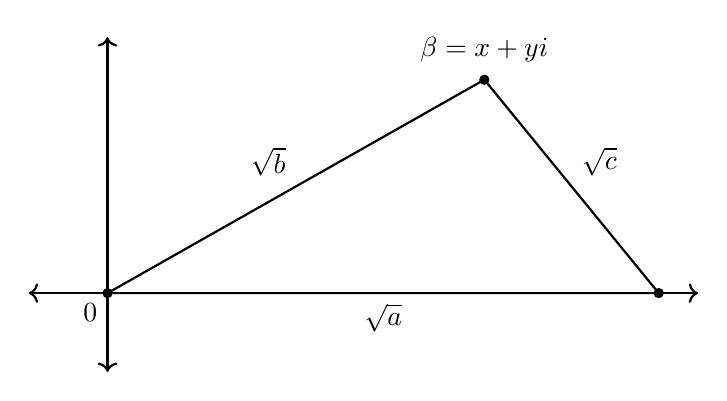
\begin{tikzpicture}[thick,scale=1, every node/.style={scale=1}]
    
  
  % Draw axes
  \draw[thick,<->] (-1,0) -- (7.5,0);
  \draw[thick,<->] (0,-1) -- (0,3.25);
  
  
  % Draw triangle
  \draw[thick] (0,0) -- (7,0) -- (4.78571428,2.710523708) -- (0,0);
  
  % Plot and label vertices
  	% Origin
  \draw[fill] (0,0) circle (.5mm);
  \draw (0,0) node[below left] {$0$};
  
  	% Right vertex
  \draw[fill] (7,0) circle (.5mm);
  \draw (3.5,0) node[below] {$\sqrt{a}$};
  
  	% Top vertex
  \draw[fill] (4.7857142,2.7105) circle (.5mm);
  \draw (4.7857142,2.8105237) node[above] {$\beta = x + yi$};
  \draw (4.7857142/2,2.7105237/2) node[above left] {$\sqrt{b}$};
  \draw (11.7857142/2,2.7105237/2) node[above right] {$\sqrt{c}$};
  
  \end{tikzpicture}
  \end{center}
  \end{figure}

Assuming the characteristic $D$ of $\M$ is defined, let $\beta = x + yi \in \M$ be any point of $\M$ not on the real axis.  The area of the triangle formed by $\alpha$ and $\beta$ with the origin is of the form $\frac{z}{4}\sqrt{D}$ for some positive integer $z$.  The above figure is just one possible configuration this triangle may have.  However, $\beta$ could potentially lie to the right of $\sqrt{a}$ or even in another quadrant.  Still, regardless of where $\beta$ lies, the following system holds:
$$
b = x^2 + y^2, \hspace{1cm} c = (x-\sqrt{a})^2 + y^2, \hspace{1cm} y^2 = \dfrac{z^2D}{4a}
$$
The first two equations come only from the Pythagorean theorem and the last from the standard formula for the area of a triangle.  From these, we deduce
\begin{align*}
x = \frac{a+b-c}{2\sqrt{a}} \hspace{1.5cm}
y = \pm \frac{z\sqrt{D}}{2\sqrt{a}}
\end{align*}
The first equality is obtained by manipulating the first two equations given just prior to these.  Therefore,
\begin{align*}
\varphi(\beta) = \frac{a+b-c}{2\sqrt{a}}\frac{\alpha}{\sqrt{a}} \pm \frac{z\sqrt{D}}{2\sqrt{a}}\frac{\alpha \delta}{\sqrt{aD}} = \frac{a+b-c}{2a}\alpha \pm \frac{z}{2a} \alpha \delta \in Q.
\end{align*}
Since $\beta$ was an arbitrary point of $\M$ not on the real axis, $\varphi$ embeds the entire set $\M$ into $Q$.
\end{proof}

We will need one final lemma before proving the main theorem.

\begin{lem} \label{lem:odd}
\normalfont
Let $T$ be a triangle of characteristic $D$ with sidelengths $\sqrt{a}, \sqrt{b}$, and $\sqrt{c}$, and suppose $D \not \equiv 3 \pmod{4}$.  Then $a+b-c$ is even, and when the area of $T$ is written as $\frac{z}{4}\sqrt{D}$, $z$ is even as well.
\end{lem}
\begin{proof}
Suppose $a+b-c$ is odd.  Then either one or all three of these terms are odd.  By Heron's formula, we have
$$
z^2D = -(a^2 + b^2 + c^2) + 2(ab+ac+bc).
$$
If $a$ is odd but $b$ and $c$ are even, then $-(a^2 + b^2 + c^2) \equiv 3 \pmod{4}$ and $2(ab+ac+bc) \equiv 0 \pmod{4}$.  If $a$, $b$, and $c$ are all odd, then $-(a^2 + b^2 + c^2) \equiv 1 \pmod{4}$ and $2(ab+ac+bc) \equiv 2 \pmod{4}$.  Either way, we have $z^2D \equiv 3 \pmod{4}$.  Since $z^2 \equiv 0$ or $1 \pmod{4}$, we must have $D \equiv 3 \pmod{4}$ since $z^2 \equiv 0$ would be a contradiction.

Now, assuming $D \not \equiv 3 \pmod{4}$, we now know that $a+b-c$ is even, and thus either one of the terms is even or all of them are.  By a similar analysis, one checks that $z^2D$ is divisible by $4$.  $D$ being squarefree, this means that $z^2$ and therefore $z$ is even.
\end{proof}

\begin{thm} \label{thm:planquatemb}
\normalfont
Let $\M$ be a planar integer norm set with characteristic $D$.
\begin{enumerate}
\item If $D \not \equiv 7 \pmod{8}$, then $\M$ embeds in $\HH$.
\item If $D \not \equiv 3 \pmod{4}$ then $\M$ embeds in $\L$.
\end{enumerate}
\end{thm}

\begin{proof}
In both of these situations, Proposition~\ref{prop:quatratemb} ensures that $\M$ embeds in $\Q(i,j)$.  Therefore, by Theorem~\ref{thm:quatemb} we know that $\M$ embeds in $\HH$ in both cases.  Now, suppose that $D \not \equiv 3 \pmod{4}$.  We may assume $\M$ is finite, since it certainly has a finite generating set.  We will also, for now, begin with the assumption that $\M$ is primitive.  From Theorem~\ref{thm:quatemb}, we realize it suffices to show that, in the embedding of $\M$ in $\Q(i,j)$ found in Proposition~\ref{prop:quatratemb}, the denominator of every point was odd.  Recall from the proof of Proposition 6 that one point of the embedding was some $\alpha \in \L$, and that every point $\gamma$ not lying on a line through $\alpha$ and the origin took the form
$$
\gamma = \frac{a+b-c}{2a}\alpha \pm \frac{z}{2a}\alpha \delta
$$
where $a = \norm{\alpha}$, $b = \norm{\gamma}$, $c = \norm{\alpha - \gamma}$, and $\delta \in \L$.  Further, $\alpha$ could be taken to be the image under the embedding of any arbitrary point in $\M$.

Since we are for now assuming $\M \subseteq \C$ to be primitive, there must be at least some pair $\alpha', \eta \in \M$ for which $\norm{\alpha' - \eta}$ is odd.  Translate and rotate $\M$ so that $\eta$ lies at the origin and $\alpha'$ lies on the real axis.  Then $a = \norm{\alpha'}$ is odd, and we may proceed to embed $\M$ in $\Q(i,j)$ with this $\alpha'$ as our choice for $\alpha$.

If $\beta$ is some point of the embedding which lies on the line passing through $\alpha$ and the origin, then $\beta = \frac{\sqrt{\norm{\beta}}}{\sqrt{\norm{\alpha}}} \alpha$.  Since $\Z[\{\alpha, \beta\}]$ is generated by a single element, we know $\beta$ is a rational multiple of $\alpha$.  Therefore, $\frac{\sqrt{\norm{\beta}}}{\sqrt{\norm{\alpha}}}$ must be rational, and so there is a positive squarefree integer $E$ such that $\norm{\alpha} = r^2E$ and $\norm{\beta} = s^2E$.  $r$ must be odd because $\norm{\alpha}$ is assumed to be odd, and thus the denominator of $\beta$ is odd because $\beta = \frac{s}{r}\alpha$.

Now, suppose $\gamma$ is a point not on a line through the embedded image of $\alpha$ and the origin.  The triangle formed by $\alpha$ and $\gamma$ with the origin has characteristic $D \not \equiv 3 \pmod{4}$.  Thus, by Lemma~\ref{lem:odd}, $a+b-c$ and $z$ are both even in the expression
$$
\dfrac{\frac12 (a+b-c \pm z\delta)\alpha}{a}
$$
hence both the numerator and denominator are in $\L$.  Thus, all points have odd denominators, so $\M$ embeds in $\L$.

If $\M$ is not primitive, then scale $\M$ down by some factor $\frac{1}{\sqrt{d}}$ to obtain a primitive integer norm set, which we may then embed in $\L$.  Now, left multiply this embedding of $\frac{1}{\sqrt{d}}\M$ by any Lipschitz quaternion of norm $d$ to retrieve an embedding of the original pointset in $\L$.
\end{proof}


The only remaining characteristics to consider are those congruent to $7 \pmod{8}$.  It is most definitely not true that these pointsets embed in the Hurwitz quaternions.  However, I have a conjecture.

\begin{conj}
\normalfont
If the characteristic of a planar integer norm set is congruent to $7 \pmod{8}$, then it embeds in the Kleinian octaves.
\end{conj}
I have verified this conjecture for all primitive integer norm triangles with a maximum diamater of $\sqrt{67}$ and maximum characteristic of $87$.  This means that all planar integer norm sets with characteristic $\leq 87$ and a basis forming a triangle with diameter $\leq \sqrt{67}$ embed in the Kleinian octaves. If this were to hold, it would mean that every integer norm triangle embeds in the double Hurwitzian ring, since this is the lattice generated by the Hurwitz integers together with the Kleinian octaves.  There are many possible approaches to proving this conjecture.  The following example is worth presenting, in case the method used can be generalized.

\begin{prop}
\normalfont
Let $T$ be an isosceles triangle with sidelengths $\sqrt{a}, \sqrt{b}, \sqrt{b}$ for positive integers $a < b$.  Then $T$ embeds in the double Hurwitz ring.
\end{prop}

\begin{proof}
By Theorem~\ref{thm:planquatemb}, the equilateral triangle with common sidelength $\sqrt{a}$ embeds in $\H$ as $\{0,\alpha, \beta\}$, since all equilateral triangles have characteristic 3.  Let $\gamma \in \H$ be any element of norm $b - a$.  Then $\{0, \alpha + i_2 \gamma, \beta + i_2\gamma\}$ is an embedding of $T$, because
$$
\norm{(\alpha + i_2\gamma) - (\beta + i_2\gamma)} = \norm{\alpha - \beta} = a
$$
and
$$
\norm{\alpha + i_2\gamma} = \norm{\alpha} + \norm{\gamma} = a + (b-a) = b = \norm{\beta} + \norm{\gamma} = \norm{\beta + i_2\gamma}.
$$
\end{proof}

This method entails partitioning the norms of the pairwise differences of a pointset in a way that forms two integer norm sets, neither of characteristic $7 \pmod{8}$, then embedding the two sets into two orthogonal copies of the Hurwitz integers.  Another path to proving this conjecture might require using a proof similar to that of Theorem~\ref{thm:planquatemb}.  This would require us to first understand the nature of factorization in the orders of $\Q(i_0,i_1,i_2)$ containing $\G$.

Unfortunately, the foundation of factorization in these orders has not yet been laid out, as it has been for the Lipschitz and Hurwitz quaternions by Pall and others.  For the Hurwitz quaternions, we have a division algorithm that we can use along with associativity to prove several familiar facts regarding factorization.  In Pall's paper, he relies heavily on the theory of quadratic forms to prove his results regarding the Lipschitz quaternions, which do not satisfy the division algorithm.  However, I imagine the complicated system of halving sets in these $8$-dimensional orders could cause this coordinate-driven approach to become complicated quickly.  The following conjecture is based more on intuition than experimentation.

\begin{conj}
\normalfont
Every integer norm set in $\Q^8$ embeds in the octavian integers.
\end{conj}


\section{Factorization in the Octavian Integers}

From here on, let $\Ord$ denote the octavian integers.  It can be shown that every point of $\R^8$ lies within $\frac{1}{\sqrt{2}}$ unit of an octavian integer \cite{Co46}.  As usual, this implies that the octavian integers also satisfy the division algorithm as stated in Theorem 2.  The lack of associativity in $\O$ prevents this theorem from being employed in the usual way to compute common divisors of maximal norm.  However, a clever algorithm due to Rehm allows us to compute all divisors of an element rather efficiently.  The following proof is from his paper \cite{Re93}.

\begin{thm}[Rehm's Algorithm]
\normalfont
Let $\alpha \in \Ord$, and suppose $\norm{\alpha} = mn$.  Then $\alpha$ has a left and a right divisor of norm $m$.
\end{thm}

\begin{proof}
Induct on $n$.  This is clear if $m=0$, so assume otherwise.  We may write
$$
\alpha = m\delta + \rho
$$
with $\norm{\rho} \leq \frac{m^2}{2}$.  Also,
$$
\norm{\rho} = \norm{\alpha} + m^2\norm{\delta} - 2m\norm{\delta, \alpha}
$$
and $m$ divides each term on the righthand side, therefore $m$ divides $\norm{\rho}$.  So, if $\frac{m^2}{2} < mn$, then we know $\norm{\rho} = mn'$ for some $n' < n$, hence by the inductive hypothesis we can write $\rho = \theta \gamma$ with $\norm{\theta} = m$.  Thus,
$$
\alpha = m\delta + \rho = (\theta \bar{\theta})\delta + \theta \gamma = \theta(\bar{\theta}\delta) + \theta \gamma = \theta(\bar{\theta}\delta + \gamma)
$$
and so $\alpha$ has a lefthand divisor of norm $m$, as desired.  Note here that we have used the fact that $\O$ is alternative in order to complete this factorization.  Since $\bar{\theta}$ is in the algebra generated by $\delta$ and $\theta$, we have $(\theta \bar{\theta})\delta = \theta(\bar{\theta}\delta)$.  Finally, factoring $\rho$ with a righthand factor of norm $m$ similarly gives a factorization of $\alpha$ with a righthand factor of norm $m$.

It will not always be the case that $\frac{m^2}{2} < mn$.  If this does not happen, then we can instead factor $\alpha$ as
$$
\alpha = \delta'n + \rho'
$$
with $\norm{\rho'} \leq \frac{n^2}{2}$.  We must now have $\frac{n^2}{2} < mn$, and so $\rho = \gamma ' \theta '$ with $\norm{\theta'} = n$.  Thus,
$$
\alpha = (\delta' \bar{\theta'} + \gamma') \theta'
$$
is a factorization where the lefthand factor has norm $m$.  We produce a righthand factor in a similar manner.
\end{proof}

If this algorithm is carried out in more detail, it can actually be shown that the set of lefthand (resp. righthand) divisors of $\alpha$ of norm $m$, if $\alpha$ is coprime to $m$, is geometrically similar to the set of $240$ octavian units.  More formally, there are isometries $\phi_L$ and $\phi_R$ of $\O$ such that the set of lefthand (resp. righthand) divisors of $\alpha$ of norm $m$ is the image of the set of all 240 octavian units under the map $m \cdot \phi_L$ (resp. $m\cdot \phi_R$).  Furthermore, if we let $d$ be the greatest common rational divisor of $\alpha$, $m$, and $n$, then the sets of left and right divisors of $\alpha$ of norm $m$ are geometrically similar to the set of all elements of norm $d$ \cite{Co03}.  Regarding the common divisors of two elements, all I have to offer is the following conjecture.

\begin{conj}
\normalfont
Let $\alpha$ and $\beta$ be octavian integers such that $p \mid \norm{\alpha}, \norm{\beta}, 2\norm{\alpha, \beta}$ for some prime $p$.  Then $\alpha$ and $\beta$ share either a left or a right divisor of norm $p$.
\end{conj}
Suppose $\alpha$ and $\beta$ satisfy the hypothesis of this conjecture.  If either of $\alpha$ or $\beta$ is divisible by $p$, this conjecture is obviously true.  For if $p \mid \alpha$ and $\theta$ is a left divisor of $\beta$ of norm $p$, then $\alpha = p\alpha' = (\theta \bar{\theta})\alpha' = \theta(\bar{\theta}\alpha')$ has a left divisor of $\theta$ as well.  Therefore, the only case with any substance is that where both $\alpha$ and $\beta$ are proper $\pmod{p}$.  It cannot be said, as it can in the case of the Lipschitz quaternions, that $\alpha$ and $\beta$ actually share all of their left or right divisors.  Consider the following counterexample, also given in vector notion.
\begin{align*}
\alpha' &= (1,1,0,0,0,0,0,1) = i_\infty + i_0 + i_6 \\
\beta'  &= (0,1,0,0,1,2,0,1) = i_0 + i_3 + 2i_4 + i_6 \\
\theta  &= (2,2,3,6,4,2,0,8) = 2i_\infty + 2i_0 + 3i_1 + 6i_2 + 4i_3 + 2i_4 + 8i_6
\end{align*}
Let $\alpha = \theta \alpha'$ and $\beta = \theta\beta'$.  We have $\norm{\alpha'} = 3$, $\norm{\beta'} = 7$, and $\norm{\theta} = 137$.  Clearly, $137$ divides $2\norm{\alpha,\beta} = 2\norm{\theta}\norm{\alpha',\beta'}$.  However, $\alpha$ and $\beta$ share no common right divisors of norm $137$, and $\theta$ and $-\theta$ are their only common left divisors.  Examples like this seem to become more likely when $p$ is large relative to $\norm{\alpha}$ and $\norm{\beta}$.

\vspace{7cm}

















\pagebreak

\section{Appendix: Consequences of the Composition Law}
Recall the defining feature of a composition algebra $A$ is that the norm is multiplicative.  We have also defined two other symbols, namely the conjugation operator
$$
\bar{\alpha} = 2 \norm{\alpha, 1} - \alpha
$$
and, $\alpha \neq 0$, the inverse operator
$$
\alpha^{-1} = \frac{\bar{\alpha}}{\norm{\alpha}}.
$$
We will soon see that this operator does in fact give an inverse.  The norm can be related to the inner product by
$$
\norm{\alpha,\beta} = \frac{\norm{\alpha + \beta} - \norm{\alpha} - \norm{\beta}}{2}.
$$
From the axioms of a composition algebra alone, we are able to determine several useful properties.  In listing these laws below, I adhere to the naming conventions established by Conway and Smith whenever possible.  The proofs of these laws taken from their book \cite{Co03}, with some minor adjustments.  In situations where a proposition involves a statement involving a left multiplication as well as a symmetric version of the statement using right multiplication, I will only prove one of the statements, since the proof of the other would be redundant.  Note that $\alpha = \beta$ if and only if $\norm{\alpha, \omega} = \norm{\beta, \omega}$ for all $\omega$, since the only vector orthogonal to the entire space is $0$.
\subsection{The Multiplication Laws}
\begin{enumerate}
\item[(M1)] \textbf{The Composition Law:}
$
\norm{\alpha \beta} = \norm{\alpha}\norm{\beta}
$

\item[(M2)] \textbf{The Scaling Laws:}
$
\norm{\alpha\beta, \alpha \gamma} = \norm{\alpha}\norm{\beta,\gamma}
$
and
$
\norm{\beta\alpha, \gamma\alpha} = \norm{\beta,\gamma}\norm{\alpha}
$

\begin{proof}
$
\norm{\alpha \beta, \alpha \gamma}
=
\dfrac{\norm{\alpha\beta + \alpha \gamma} - \norm{\alpha\beta} - \norm{\alpha \gamma}}{2}
\overset{\text{M}1}{=}
\norm{\alpha}\dfrac{\norm{\beta + \gamma} - \norm{\beta} - \norm{\gamma}}{2} = \norm{\alpha}\norm{\beta,\gamma}.
$
\end{proof}

\item[(M3)] \textbf{The Exchange Law:}
$ \norm{\alpha \beta, \gamma \delta} = 2 \norm{\alpha, \gamma}\norm{\beta, \delta} - \norm{\alpha \delta, \gamma \beta}$.

\begin{proof}
We have
\begin{align*}
\norm{\alpha \beta, \alpha \delta} + 2\norm{\alpha, \gamma}\norm{\beta,\delta} + \norm{\gamma\beta, \gamma \delta}
&\overset{\text{M}2}{=}
(\norm{\alpha} + 2\norm{\alpha,\gamma} + \norm{\gamma})\norm{\beta,\delta}
\\
&\overset{\phantom{\text{M}2}}{=}
\norm{\alpha + \gamma}\norm{\beta,\delta}
\\
&\overset{\text{M}2}{=} \norm{(\alpha + \gamma)\beta, (\alpha + \gamma)\delta}
\\
&\overset{\phantom{\text{M}2}}{=}
\norm{\alpha\beta, \alpha\delta} + \norm{\alpha \beta, \gamma \delta} + \norm{\gamma\beta,\alpha\delta} + \norm{\gamma\beta, \gamma\delta}
\end{align*}
thus
\begin{align*}
\norm{\alpha \beta, \gamma \delta}
&=
(\norm{\alpha\beta, \alpha\delta} + \norm{\alpha \beta, \gamma \delta} + \norm{\gamma\beta,\alpha\delta} + \norm{\gamma\beta, \gamma\delta})
-
(\norm{\alpha\beta, \alpha\delta} + \norm{\gamma\beta,\alpha\delta} + \norm{\gamma\beta, \gamma\delta})
\\
&=
(\norm{\alpha \beta, \alpha \delta} + 2\norm{\alpha, \gamma}\norm{\beta,\delta} + \norm{\gamma\beta, \gamma \delta})
-
(\norm{\alpha\beta, \alpha\delta} + \norm{\gamma\beta,\alpha\delta} + \norm{\gamma\beta, \gamma\delta})
\\
&=
2\norm{\alpha, \gamma}\norm{\beta,\delta}
-
\norm{\alpha\delta,\gamma\beta}.
\end{align*}

\end{proof}

\end{enumerate}

\subsection{The Conjugation Laws}
\begin{enumerate}
\item[(C1)] \textbf{The Braid Laws:}
$
\norm{\alpha \beta, \delta} = \norm{\beta, \bar{\alpha}\delta}$ and $\norm{ \alpha, \beta \delta} = \norm{\bar{\beta} \alpha , \delta }
$

\begin{proof}
We make the substitution $\gamma = 1$ in M3:
\begin{align*}
\norm{\beta, \bar{\alpha}\delta}
=
\norm{\beta, (2\norm{\alpha,1} - \alpha)\delta}
=
2\norm{\alpha,1}\norm{\beta,\delta} - \norm{\beta,\alpha\delta}
\overset{\text{M}3}{=} \norm{\alpha\beta,\delta}.
\end{align*}
\end{proof}

\item[(C2)] \textbf{Biconjugation:}
$
\bar{\bar{\alpha}} = \alpha
$

\begin{proof}
For all $\omega \in A$,
$$
\norm{\alpha, \omega} \overset{\text{C}1}{=} \norm{1, \bar{\alpha}\omega} \overset{\text{C}1}{=} \norm{\bar{\bar{\alpha}},\omega}.
$$
\end{proof}

\item[(C3)] \textbf{Product Conjugation:}
$\bar{\alpha \beta} = \bar{\beta}\bar{\alpha}$

\begin{proof}
For all $\omega \in A$,
$$
\norm{\bar{\beta}\bar{\alpha},\omega} = \norm{\bar{\alpha},\beta\omega} = \norm{\bar{\alpha} \ \bar{\omega},\beta} = \norm{\bar{\omega},\alpha \beta} = \norm{\bar{\omega}\bar{\alpha \beta},1} = \norm{\bar{\alpha\beta},\omega}
$$
where every equality follows from C1.
\end{proof}

\item[(C4)] \textbf{Equivalent Definition of Norm:}
$\norm{\alpha} = \alpha \bar{\alpha}$

\begin{proof}
For all $\omega \in A$,
$$
\norm{\alpha \bar{\alpha},\omega} \overset{\text{C}1}{=} \norm{\alpha, \alpha \omega} \overset{\text{M}2}{=} \norm{\alpha}\norm{1, \omega} = \norm{\norm{\alpha},\omega}.
$$
\end{proof}
\noindent
From this last law, it also becomes clear that our inverse operator truly outputs the multiplicative inverse of its argument.  We also have $\norm{\bar{\alpha}} = \norm{\bar{\alpha},\bar{\alpha}} \overset{\text{C}1}{=} \norm{1,\alpha\bar{\alpha}} \overset{\text{C}4}{=} \norm{1,\norm{\alpha}} \overset{\text{M}2}{=} \norm{1,1} \norm{\alpha} = \norm{\alpha}$.
\end{enumerate}

\subsection{The Semi-Associativity Laws}
\begin{enumerate}
\item[(S1)] \textbf{Inverse Laws:}
$
\bar{\alpha}(\alpha\beta) = \norm{\alpha}\beta = (\beta \alpha)\bar{\alpha}
$
and
$
\alpha^{-1}(\alpha\beta) = \beta = (\beta \alpha)\alpha^{-1}
$

\begin{proof}
For all $\omega \in A$,
$$
\norm{\bar{\alpha}(\alpha\beta),\omega} \overset{\text{C}1}{=} \norm{\alpha \beta, \alpha \omega} \overset{\text{M}2}{=} \norm{\alpha}\norm{\beta, \omega} = \norm{\norm{\alpha}\beta, \omega} \overset{\text{C}4}{=} \norm{(\alpha \bar{\alpha})\beta,\omega}.
$$
The latter statement results from dividing the former by $\norm{\alpha}$.
\end{proof}

\item[(S2)] \textbf{Alternative Laws:}
$\alpha(\alpha\beta) = \alpha^2 \beta$ and $(\alpha \beta)\beta = \alpha\beta^2$

\begin{proof}
\begin{align*}
\alpha(\alpha \beta)
&\overset{\phantom{\text{S}1}}{=}
2\norm{\alpha,1}\alpha\beta - (2\norm{\alpha,1}\alpha\beta - \alpha(\alpha \beta))
\\
&\overset{\phantom{\text{S}1}}{=}
2\norm{\alpha,1}\alpha\beta - \bar{\alpha}(\alpha\beta)
\\
&\overset{\text{S}1}{=}
2\norm{\alpha,1}\alpha\beta - (\bar{\alpha}\alpha)\beta
\\
&\overset{\phantom{\text{S}1}}{=}
2\norm{\alpha,1}\alpha\beta - ((2\norm{\alpha,1}-\alpha)\alpha)\beta
\\
&\overset{\phantom{\text{S}1}}{=}
\alpha^2\beta
\end{align*}
\end{proof}

\item[(S3)] \textbf{Moufang Laws:}
$(\alpha \beta)(\gamma \alpha) = (\alpha(\beta \gamma))\alpha = \alpha((\beta \gamma)\alpha)$

\begin{proof}
For all $\omega \in A$,
\begin{align*}
\norm{(\alpha\beta)(\gamma\alpha),\omega}
&\overset{\text{C}1}{=} \norm{\alpha\beta, \omega(\bar{\gamma\alpha})}
\\
&\overset{\text{C}3}{=} \norm{\alpha\beta, \omega(\bar{\alpha} \ \bar{\gamma})}
\\
&\overset{\text{M}3}{=} 2\norm{\alpha,\omega}\norm{\beta,\bar{\alpha} \ \bar{\gamma}} - \norm{\alpha(\bar{\alpha} \ \bar{\gamma}),\omega\beta}
\\
&\overset{\text{C}1}{=} 2\norm{\alpha,\omega}\norm{\beta\gamma,\bar{\alpha}} - \norm{\bar{\alpha} \ \bar{\gamma}, \bar{\alpha}(\omega \beta)}
\\
&\overset{\text{M}2}{=} 2\norm{\alpha,\omega}\norm{\beta\gamma,\bar{\alpha}} - \norm{\alpha}\norm{\bar{\gamma} \ \bar{\beta}, \omega}
\\
&\overset{\text{C}3}{=}
\norm{2\norm{\beta\gamma,\bar{\alpha}}\alpha - \norm{\alpha}\bar{\beta \gamma} , \omega}
\end{align*}
thus $(\alpha\beta)(\gamma\alpha) = 2\norm{\beta\gamma,\bar{\alpha}}\alpha - \norm{\alpha}\bar{\beta \gamma}$.  Therefore, this expression is a function of the product $\beta \gamma$, and does not depend on the individual factors $\beta$ and $\gamma$.  Thus, we may replace $\beta$ with $\beta\gamma$ and $\gamma$ with $1$ (or vice versa), giving the result.
\end{proof}

\end{enumerate}

\subsection{The Doubling Laws}
Let $H$ be a subalgebra of $A$, let $i \in H$ be a unit vector orthogonal to $A$, and let $\alpha, \beta, \gamma, \delta \in H$.
\begin{enumerate}
\item[(D1)] \textbf{Inner-Product Doubling:}
$
\norm{\alpha + i\beta, \gamma + i \delta} = \norm{\alpha, \gamma} + \norm{\beta, \delta}
$

\begin{proof}
\begin{align*}
\norm{\alpha + i\beta, \gamma + i \delta}
&\overset{\text{M2}}{=}
\norm{\alpha, \gamma} + \norm{\alpha, i\delta} + \norm{i\beta, \gamma} + \norm{i}\norm{\beta, \delta}
\\
&\overset{\text{C1}}{=} \norm{\alpha, \gamma} + \norm{\alpha\bar{\delta}, i} + \norm{i, \gamma \bar{\beta}} + \norm{i}\norm{\beta,\delta}
\\
&\overset{\phantom{\text{M}2}}{=}
\norm{\alpha, \gamma} + \norm{\beta,\delta}.
\end{align*}
\end{proof}

\item[(D2)] \textbf{Conjugation Doubling:}
$
\bar{\alpha + i \beta} = \bar{\alpha} - i\beta
$

\begin{proof}
$$
\bar{\alpha + i\beta} = 2\norm{\alpha,1} + 2\norm{i\beta,1} - \alpha - i\beta \overset{\text{C1}}{=} \bar{\alpha} - i\beta - 2\norm{i,\bar{\beta}} = \bar{\alpha} - i\beta
$$
\end{proof}
\noindent
Note that this also gives us $i\beta = -\bar{i \beta} = -\bar{\beta} \bar{i} = -\bar{\beta}(-i) = \bar{\beta}i$.
\item[(D3)] \textbf{Composition Doubling:}
$(\alpha + i\beta)(\gamma + i\delta) = (\alpha \gamma - \delta \bar{\beta}) + i(\gamma \beta + \bar{\alpha}\delta)$

\begin{proof}
Expanding gives
$$
(\alpha + i\beta)(\gamma + i\delta) = \alpha \gamma + (i\beta)\gamma + \alpha(i\delta) + (i\beta)(i\delta).
$$
We evaluate the final three terms:
$$
\norm{(i\beta)\gamma,\omega} \overset{\text{C}1}{=}
\norm{i\beta, \omega \bar{\gamma}}
\overset{\text{D}2}{=}
\norm{\bar{\beta}i,\omega \bar{\gamma}}
\overset{\text{M}3}{=}
0 - \norm{\bar{\beta}\ \bar{\gamma},\omega i}
\overset{\text{C1,D2}}{=}
\norm{(\bar{\beta} \ \bar{\gamma})i,\omega}
\overset{\text{D}2}{=}
\norm{i(\gamma \beta),\omega}
$$
$$
\norm{\alpha(i\delta),\omega}
\overset{\text{C}1}{=}
\norm{i\delta,\bar{\alpha}\omega}
\overset{\text{M}3}{=}
0 - \norm{i\omega,\bar{\alpha}\delta}
\overset{\text{C}1}{=}
\norm{\omega,i(\bar{\alpha}\delta)}
=
\norm{i(\bar{\alpha}\delta),\omega}
$$
$$
\norm{(i\beta)(i\delta),\omega}
\overset{\text{C1,D2}}{=}
-\norm{i\beta,\omega(i\delta)}
\overset{\text{M}3}{=}
0 + \norm{i(i\delta),\omega\beta}
\overset{\text{S2}}{=}
-\norm{\delta,\omega\beta}
\overset{\text{C}1}{=}
\norm{-\delta\bar{\beta},\omega}
$$
This gives
$$
(\alpha + i\beta)(\gamma + i\delta) = \alpha \gamma + i(\gamma\beta) + i(\bar{\alpha}\delta) - \delta \bar{\beta} = (\alpha\gamma - \delta \bar{\beta}) + i(\gamma\beta + \bar{\alpha}\delta).
$$
\end{proof}

\end{enumerate}


\begin{comment}
\subsection{$ij=k$}

We are all probably familiar with the story of William Rowan Hamilton's discovery of the quaternion multiplication laws, and his subsequent carving of these anticommutative relations into the side of a bridge.  Hamilton had, essentially, been in search of an extension of $\C$ to a higher dimensional composition algebra.  The relations which he discovered are not only in no way arbitrary, but actually necessary.  In the next paragraph, I derive these relations from the composition law.  This demonstration is technically not necessary, since the Doubling Laws dictate that we have no choice in defining the multiplication on the Dickson double of an algebra.  Therefore, if $\R = A_0 \subsetneq A_1 \subsetneq A_2 \subsetneq A_3$ is a chain of composition algebras for which no other algebra $B$ satisfies $A_s \subsetneq B \subsetneq A_t$, then $A_1 \cong \C$, $A_2 \cong \H$, and $A_3 \cong \O$.  So this discussion should be seen as a concrete demonstration of how the algebra resulting from composition doubling is determined.

For an explicit derivation of the quaternion multiplicative relations, suppose $H$ is a composition algebra containing $\C$, and take $j\in H$ to be a unit vector orthogonal to $\C$.  First, we see that if $\omega \in H$ then $\norm{ij, \omega} \overset{\text{C}1}{=} -\norm{j,i\omega} = 0$ and also $\norm{ij,j} \overset{\text{M}2}{=} \norm{i,1}\norm{j} = 0$.  Thus $k = ij$ is orthogonal to $H + \R j$.  Also, by (D3) we have $j^2 = -1$.  Next, we have for all $\omega \in H$ that
$$
\norm{(ij)i,\omega} \overset{\text{C}1}{=}
-\norm{ij,\omega i} \overset{\text{M}3}{=}
-2\norm{i,\omega}\norm{j,i} + \norm{i^2,\omega j}
= -2\norm{i,\omega}\cdot 0 - \norm{1,\omega j}
\overset{\text{C}1}{=} \norm{j,\omega}.
$$
So $(ij)i = j$.  A right multiplication by $i$, followed by a right multiplication by $j$, gives $(ji)j = i$ as well.  We also have $j(ij) \overset{\text{D3}}{=} i$.  Therefore, $jk = j(ij) = i$ and $ki = (ij)i = j$.  Conjugating these relations gives $kj = -i$ and $ik = -j$, and conjugating $ij = k$ gives $-ji = k$.  We also have $j^2 \overset{\text{D3}}{=} -1 \overset{\text{D3}}{=} k^2$.
\end{comment}

\begin{comment}
\subsection{Diassociativity}
Here, we prove a statement that is stronger than Artin's theorem in the case of the octonion algebra.  The proof builds on ideas from the section on Composition Algebras, which should be read prior to reading this section.
\begin{thm}
The subalgebra generated by any two elements of $\O$ is isomorphic to $\C$ or to $\H$.  In particular, it is associative.
\end{thm}
\begin{proof}
Let $\alpha, \beta \in \O$.  First, suppose $\beta \not \in \R(\alpha)$.  There exist $i',j' \in \O$ such that $\{1,i',j',i'j'\}$ is an orthonormal basis for $\R(\alpha,\beta)$.  To see this, apply Gram-Schmidt to a basis for $\R(\alpha,\beta)$ that includes $1$, obtaining a basis of the form $\{1,i',j',k'\}$.  Now, replace $k'$ with $i'j'$, since we know it must be orthogonal to the $1$, $i'$, and $j'$ and have unit norm.  An isomorphism from $\H$ to $\R(\alpha,\beta)$ is given by $i \mapsto i', j \mapsto j'$, since in the Cayley-Dickson construction, $i$ could have been taken to be $i'$ in the construction of $\C$ from $\R$, and likewise $j$ could have been taken to be $j'$ in the construction of $\H$ from $\C$, since all that is required of these vectors is that they are orthogonal to the space which we are ``doubling."  By similar reasoning, we see that if $\beta \in \R(\alpha)$ then $\R(\alpha,\beta) = \R(\alpha) \cong \C$.
\end{proof}
\end{comment}

\begin{comment}
\subsection{Generalized Permuations}
Let $A$ be an algebraic structure with one binary operation and an inverse operator, written additively. Let $I$ be an index set.  A \emph{generalized permutation} is an operation on $\prod_{t \in I} A$ of the form
$$
\prod_{t \in I} x_i \mapsto \prod_{t \in I}\lambda_t (x_{\sigma^{-1}(t)})
$$
where $\lambda: I \rightarrow \{\text{id}, x \mapsto -x\}$ assigns, to each element $t \in I$, a function $\lambda_t$ which is either the identity map on $A$ or the inverse map on $A$, and $\sigma$ is a permutation of $I$.  Less formally, a generalized permutation is an operation on $\prod_{t \in I} A$ that permutes components change signs.  For a given generalized permutation, we will call the $\sigma$ referred to above the \emph{associated permutation}.  Our reason for using $\sigma^{-1}$ in the definition rather than $\sigma$ will hopefully be made clear by this example: $(a,b,c) \mapsto (-c,a,b)$ is a generalized permutation on $A^3$ with $\lambda$ defined by $1 \mapsto (x \mapsto -x)$, and $2,3 \mapsto \text{id}$, and associated permutation defined by $1 \rightarrow 2 \rightarrow 3 \rightarrow 1$.  It is more natural for us to think, for instance, ``$a$ goes from the first component to the second," than ``the entry that is now in the second component is the one that was before in the first."  If $f$ and $g$ are two generalized permutations on $\prod_{t \in I} A$, and the associated permutations are $\sigma$ and $\tau$, respectively, then $\sigma\tau = \sigma \circ \tau$ is the permutation associated with $f \circ g$.

Let $\Omega = \{\infty,0,1,2,3,4,5,6\}$, so that $\O \cong \prod_{t \in \Omega}\R$.  Every element $\gamma \in \O$ induces left and right multiplication operators $L_\gamma$ and $R_\gamma$ on $\O$, defined in the obvious way.  If $\gamma = i_r$ for some $r \in \Omega$, then these operators are generalized permutations on $\O$ when it is viewed as $\R^8$.  Fix some $r \in \Omega$ and assume $M_{i_r}$ is one of $L_{i_r}$ or $R_{i_r}$, since the arguments we will use for one apply to both.  Note that, for $t \in \Omega$, $\sigma$ is the permutation associated with $M_{i_t}$ if and only if
$$
M_{i_t}\left( \sum_{s \in \Omega} a_s i_s \right) = \sum_{s \in \Omega} a_{\sigma^{-1}(s)} i_s = \sum_{s \in \Omega} a_s i_{\sigma(s)}.
$$



Now, if $r \neq \infty$ and $s \in \Omega \setminus \{\infty, r\}$, then $M_{i_r}$ is a generalized permutation on the quaternion subalgebra generated by $i_r$ and $i_s$.  However, if $S$ is a 4-element subset of $\Omega$ such that $\R(\{i_t : t \in S\}) \cong \H$ and $r \in S^c = \Omega \setminus S$, then $\sigma(S) = S^c$ and $\sigma(S^c) = S$.  To see this, first check the claim for $S = \{ \infty, 0, 1, 3\}$ and $r = 2$:

\begin{align*}
L_{i_2}(a i_\infty +  b i_0 + c i_1 + d i_3) &= ai_2 - bi_6 - ci_4 + d i_5 \\
R_{i_2}(a i_\infty +  b i_0 + c i_1 + d i_3) &= ai_2 + bi_6 + ci_4 - d i_5
\end{align*}

If $S'$ is another 4-element subset of $\Omega$ such that $\R(\{i_t : t \in S'\}) \cong \H$ and $r' \not \in S$, then by Theorem~\ref{thm:autom} there is a permutation $\tau$ of $\Omega$ taking $S'$ to $S$ (note that this implies $\tau(S'^c) = S^c$ as well) and $r'$ to $r$ that induces an automorphism $\varphi_{\tau}$ of $\O$, defined by
$$
\varphi_{\tau}\left( \sum\limits_{s \in \Omega} a_s i_s \right) = \sum\limits_{s \in \Omega} a_s i_{\tau(s)}.
$$
$\varphi_{\tau}$ is also a generalized permutation on $\O$, with associated permutation $\tau$.  Also, $\varphi_{\tau}^{-1} = \varphi_{\tau^{-1}}$ has associated permutation $\tau^{-1}$.
We now have the following commutative squares

$$
\begin{tikzpicture}[baseline= (a).base]
\node[scale=1.3] (a) at (0,0){

\begin{tikzcd}
\O \arrow{dd}[swap]{M_{i_{\tau(r)}}} \arrow{rr}{\varphi_\tau} & & \O \arrow{dd}{M_{i_{r}}} \\
& & & \\
\O \arrow{rr}[swap]{\varphi_\tau} & & \O
\end{tikzcd}

};


\begin{scope}[shift={(7,0)}]
\node[scale=1.3] (a) at (0,0){

\begin{tikzcd}
S' \arrow{dd}[swap]{\tau^{-1}  \sigma  \tau} \arrow{rr}{\tau} & & S \arrow{dd}{\sigma} \\
& & & \\
S'^c \arrow{rr}[swap]{\tau} & & S^c
\end{tikzcd}
};
\end{scope}
\end{tikzpicture}
$$
The commutativity of the left diagram follows from
$$
\varphi_{\tau}\circ L_{i_r} ( \alpha) = \varphi_{\tau}(i_r \alpha) = \varphi_{\tau}(i_r)\varphi_{\tau}(\alpha) = i_{\tau(r)} \varphi_\tau(\alpha) = L_{i_{\tau(r)}}\circ \varphi_\tau (\alpha)
$$
and
$$
\varphi_{\tau}\circ R_{i_r} ( \alpha) = \varphi_{\tau}(\alpha i_r) = \varphi_{\tau}(\alpha)\varphi_{\tau}(i_r) = \varphi_\tau(\alpha) i_{\tau(r)} = R_{i_{\tau(r)}}\circ \varphi_\tau (\alpha)
$$
The associated permutation of $M_{i_{\tau(r)}} = \varphi_{\tau}^{-1} \circ M_{i_r} \circ \varphi_{\tau}$ is $\tau^{-1}\sigma\tau$, which has the desired properties $\tau^{-1}\sigma\tau(S') = S'^c$ and $\tau^{-1}\sigma\tau(S'^c) = S'$.  Therefore, the proposition holds for an arbitrary halving set $S$ and $r \in S^c$.
\end{comment}
\pagebreak

\nocite{*}
\bibliographystyle{plain}
\bibliography{bib}

\end{document}














